% ---------------------------------------------------------------------
% --- Arquivo principal e os demais serao os dos capitulos.
% --- EXPRESSÕES ENTRE <> DEVERÃO SER COMPLETADAS COM A INFORMAÇÃO ESPECÍFICA DO TRABALHO 
% ---------------------------------------------------------------------

\documentclass[ruledheader]{abnt_UFF}

%---pacotes para hiphenizacao e acentuacao em portugues
\usepackage[utf8]{inputenc}
\usepackage[brazilian]{babel}
%\usepackage[latin1]{inputenc}
\usepackage[T1]{fontenc}
%--- pacote para figuras
\usepackage{epsf}
\usepackage[dvips]{epsfig,graphicx}
%\usepackage{subfigure}
\usepackage{subfig}
\usepackage{cite}
\usepackage{textcomp}
\usepackage{caption}
\usepackage{subcaption}
%--- pacote de simbolos
\usepackage{latexsym}
\usepackage{textcomp}

%--- simbolos matematicos
\usepackage{amsmath}
\usepackage{amssymb}

%--- pacote para gerar pseudo-codigo
\usepackage{algorithm}
\usepackage{algorithmic}
\floatname{algorithm}{Algoritmo}

%--- outros pacotes
\usepackage{url}
\usepackage{longtable}
\usepackage{lscape}
\usepackage{amsthm}
\usepackage{todonotes}
\usepackage{verbatim}
\usepackage{graphicx}


%Tabela Colorida
\usepackage{colortbl}
\usepackage{multicol}
\usepackage{multirow}
\usepackage{rotating}

%\usepackage{ulem}



%--- UML
\usepackage{tikz}
\usetikzlibrary{graphs,graphs.standard,arrows,decorations.pathmorphing,positioning,fit,shapes,calc}
\usepackage{tikz-uml}


\hyphenation{
a-de-qua-da-men-te 
di-men-sio-na-men-to 
re-qui-si-to
}
\usepackage{lscape}
\usepackage{listlang}
\lstset{basicstyle=\small}
\renewcommand{\lstlistingname}{Listagem}



%---------usando tipo de fonte padrao
\renewcommand{\ABNTchapterfont}{\bfseries\fontfamily{cmr}\fontseries{b}\selectfont}
\renewcommand{\ABNTsectionfont}{\bfseries\fontfamily{cmr}}



% --- -----------------------------------------------------------------
% --- Documento Principal.
% --- -----------------------------------------------------------------
% \usepackage[pdftex]{hyperref}
% \hypersetup{colorlinks, sitecolor=black, pdftex}
\begin{document}

% --- -----------------------------------------------------------------
% --- Titulo, abstract, dedicatorias e agradecimentos.
% --- Indice geral, lista de figuras e tabelas.
% --- -----------------------------------------------------------------

% --- -----------------------------------------------------------------
% --- Elementos usados na Capa e na Folha de Rosto.
% --- EXPRESSÕES ENTRE <> DEVERÃO SER COMPLETADAS COM A INFORMAÇÃO ESPECÍFICA DO TRABALHO
% --- E OS SÍMBOLOS <> DEVEM SER RETIRADOS 
% --- -----------------------------------------------------------------
\autor{RAFAEL HEITOR CORREIA DE MELO} % deve ser escrito em maiúsculo

\titulo{Uma Proposta de uso de Dispositivo Háptico \\para Treinamento de Anestesia raquidiana}

\instituicao{UNIVERSIDADE FEDERAL FLUMINENSE}

\orientador{Aura Conci, D.Sc.}

\local{NITERÓI}

\data{2021} % ano da defesa


\comentario{Tese de Doutorado apresentada ao Programa de Pós-Graduação em Computação da \mbox{Universidade} Federal Fluminense como requisito parcial para a obtenção do Grau de \mbox{Doutor em Computação}. Área de concentração: \mbox{Ciência da Computação}.} %preencha com a sua área de concentração


% --- -----------------------------------------------------------------
% --- Capa. (Capa externa, aquela com as letrinhas douradas)(Obrigatório)
% --- ----------------------------------------------------------------
\capa

% --- -----------------------------------------------------------------
% --- Folha de rosto. (Obrigatório)
% --- ----------------------------------------------------------------
\folhaderosto



\pagestyle{ruledheader}
\setcounter{page}{1}
\pagenumbering{roman}

% --- -----------------------------------------------------------------
% --- Termo de aprovacao. (Obrigatorio)
% --- ----------------------------------------------------------------
\cleardoublepage
\thispagestyle{empty}

\vspace{-60mm}

\begin{center}
   {\large RAFAEL HEITOR CORREIA DE MELO}\\
   \vspace{7mm}

   Uma Proposta de uso de Dispositivo Háptico \\para Treinamento de Anestesia raquidiana\\
   
  \vspace{10mm}
\end{center}

\noindent
\begin{flushright}
\begin{minipage}[t]{8cm}

Tese de Doutorado apresentada ao Programa de Pós-Graduação em Computação da Universidade Federal Fluminense como requisito parcial para a obtenção do \mbox{Grau} de Doutor em Computação. Área de concentração: \mbox{Sistemas de Computação.} %preencha com a sua área de concentração
\end{minipage}
\end{flushright}
\vspace{1.0 cm}
\noindent
Aprovada em MÊS de 2021. \\
\begin{flushright}
  \parbox{10cm}
  {
  \begin{center}
  BANCA EXAMINADORA \\
  \vspace{6mm}
  \rule{11cm}{.1mm} \\
    Profa. D.Sc. Aura Conci - Orientadora, UFF \\
    \vspace{6mm}
  \rule{11cm}{.1mm} \\
     Prof. ---------, UFF \\
   \vspace{6mm}

  \rule{11cm}{.1mm} \\
    Profa. -----------, UFF\\
    \vspace{4mm}
  \rule{11cm}{.1mm} \\
    Prof. ------------, SIGLAUniv\\
  \vspace{4mm}
  \rule{11cm}{.1mm} \\
   ------------------, SIGLAUniv \\
  %\vspace{6mm}
  \end{center}
  }
\end{flushright}
\begin{center}
 % \vspace{4mm}
  Niterói \\
  %\vspace{6mm}
  2021

\end{center}

% --- -----------------------------------------------------------------
% --- Dedicatoria.(Opcional)
% --- -----------------------------------------------------------------
\cleardoublepage
\thispagestyle{empty}
\vspace*{200mm}

\begin{flushright}
{\em 
%Dedicatória(s): Elemento opcional onde o autor presta homenagem ou dedica seu trabalho (ABNT, 2005).
Dedico este trabalho a minha esposa, Evelyn, que sempre me apoiou na direção das minhas conquistas e ao meu filho, Rafael, que, ao chegar me apresentou uma nova forma de amar. 
}
\end{flushright}
\newpage


% --- -----------------------------------------------------------------
% --- Agradecimentos.(Opcional)
% --- -----------------------------------------------------------------
\pretextualchapter{Agradecimentos}
\hspace{5mm}

Agradeço a Deus por me mostrar sempre os caminhos, mesmo nos momentos em que parece que isso não vai acontecer. 

Aos meus pais Julio e Dayse pela preocupação e apoio. Aos meus irmãos Leonardo e Julia pela amizade e companheirismo essenciais nos momentos difíceis.

Agradeço muito a minha orientadora Aura, que mesmo nos momentos de desânimo conseguiu me trazer, em palavras, motivação para seguir em frente.

Ao amigo André que foi essencial em parte dessa caminhada.

À minha família, agradeço a compreensão pelas minhas ausências e minhas desculpas nos momentos de desânimo.


% --- -----------------------------------------------------------------
% --- Resumo em portugues.(Obrigatorio)
% --- -----------------------------------------------------------------
\begin{resumo}

As anestesias raquidianas são procedimentos cegos que dependem do sentimento do médico no decorrer da inserção da agulha para correta identificação do local de aplicação do líquido anestésico. Em grande parte dos centros de treinamento a primeira experiência tátil do médico em treino tende a ser praticada em pacientes reais. Esta prática, apesar de ser efetuada sob supervisão direta, traz riscos para estes pacientes e possíveis inseguranças aos aprendizes. Técnicas alternativas de uso de \textit{phantoms} e cadáveres no treinamento oferecem uma pequena representatividade em relação às variações de pacientes reais. 
Este trabalho propõe o desenvolvimento de um ambiente virtual para simulação do procedimento que envolve anestesias raquidianas. Propõem-se considerar o procedimento de punção com \textit{feedback} tátil e visual usando técnicas de auto treinamento. As sensações táteis do médico em treinamento são simuladas no protótipo através da integração com dispositivo háptico. A geração e visualização dinâmica de modelos de corpos de pacientes baseados em altura e peso também faz parte do processo. A parte do protótipo que envolve a detecção de diferentes sensações de perfuração de tecidos foi validado por alunos da computação. O acesso a membros da comunidade médica foi comprometido pela realidade da pandemia. Finalmente, esta tese  também apresenta um modelo adaptável de um corpo de gestante que possui modelagem de todas as camadas desde a pele das costas até os ossos da coluna vertebral. As camadas de tecido mais variáveis foram modeladas de forma dinâmica de forma a permitir uma maior variabilidade de cenários de treinamento. Esta modelagem pode ainda ser utilizada em outros procedimentos que envolvam a área e camadas modeladas desenvolvidas. 

{\hspace{-8mm} \bf{Palavras-chave}}: Dispositivo háptico, Treinamento médico, Anestesia raquidiana, Ambiente virtual.

\end{resumo}

% --- -----------------------------------------------------------------
% --- Resumo em lingua estrangeira.(Obrigatorio)
% --- -----------------------------------------------------------------
\begin{abstract}

Advances in recognition technologies (e.g., speech or gesture recognition)  enable  new  user  interfaces  for  multimedia  systems.  It  is  possible  toprocess  two  or  more  combined  modes  of  user  interaction  captured  by  inputdevices or sensors in such systems. Moreover, viewers can use different inputdevices tailored to their special needs or particular intention. Another interesting feature in these systems is perceiving and identifying different users who are participating in the multimedia experience. There are technologies capable of relating user interactivity uniquely. However, DigitalTV (DTV) standard platforms do not fully support multimodal and multiuser interactionsnatively. Therefore, this work proposes an extension to the Brazilian Ginga-NCL DTV middleware to provide multimodal interaction. The Nested ContextLanguage (NCL) is extended (called NCL 4.0) to support new interaction events and multipleusers,  allowing  them  to  identify  which  user  has  interacted  with  a  DTV  ap-plication. As a proof of concept, we developed two new Ginga-NCL modulesthat adhere to our extended version, one that supports voice interaction andanother that supports gaze interaction. We developed several DTV applica-tions to evaluate our proposal and confirmed that our extended version doesnot cause overhead on Ginga-NCL event processing. Finally, this paper alsopresents  a  comparison  between  the  current  NCL  version  and  our  NCL 4.0 proposal considering performance and number of application code lines.

{\hspace{-8mm} \bf{Keywords}}: NCM, NCL, Ginga-NCL, NCL 4.0, Conceptual Model, Multimedia Authoring, Authoring Language, Multimodal Interaction, Multiuser Interaction, Multiuser Applications.

\end{abstract}

% --- -----------------------------------------------------------------
% --- Lista de figuras.(Opcional)
% --- -----------------------------------------------------------------
%\cleardoublepage
\listoffigures


% --- -----------------------------------------------------------------
% --- Lista de tabelas.(Opcional)
% --- -----------------------------------------------------------------
\cleardoublepage
%\label{pag:last_page_introduction}
\listoftables
\cleardoublepage

% --- -----------------------------------------------------------------
% --- Lista de abreviatura.(Opcional)
%Elemento opcional, que consiste na relação alfabética das abreviaturas e siglas utilizadas no texto, seguidas das %palavras ou expressões correspondentes grafadas por extenso. Recomenda-se a elaboração de lista própria para cada %tipo (ABNT, 2005).
% --- ----------------------------------------------------------------
\cleardoublepage
\pretextualchapter{Lista de Abreviaturas e Siglas}
\begin{tabular}{lcl}
AHM & : & Amsterdam Hypermedia Model;\\
CIDL & : & Control Information Description Language;\\
GUI & : & Graphical User Interface;\\
IIDL & : & Interaction Interface Description Language;\\
IoT & : & Internet Of Things;\\
KMS & : & Knowledge Management System;\\
MUI & : & Multimodal User Interface;\\
MultiSEM & : & Multimedia Sensory Effect Model;\\
NCL & : & Nested Context Language;\\
NCM & : & Nested Context Model;\\
PROMIS & : & Problem Oriented Medical Information System;\\
RDF & : & Resource Description Framework;\\
RoSE & : & Representation of Sensory Effects;\\
SEDL & : & Sensory Effect Description Language;\\
SEM & : & Sensory Effect Metadata;\\
SEVino & : & Sensory Effect Video Annotation;\\
SMIL & : & Synchronized Multimedia Integration Language;\\
SMURF & : & Sensible Media aUthoRing Factory;\\
SRGS & : & Speech Recognition Grammar Specification;\\
TEA & : & Transtorno do Espectro Autista;\\


\end{tabular}
% --- -----------------------------------------------------------------
% --- Sumario.(Obrigatorio)
% --- -----------------------------------------------------------------
\pagestyle{ruledheader}
\tableofcontents




% --- -----------------------------------------------------------------
% --- Insercao dos capitulos.
% --- -----------------------------------------------------------------
\pagestyle{ruledheader}
\setcounter{page}{1}
\pagenumbering{arabic}
\chapter{Introdução} \label{cap:cap1}

Nas anestesias raquidianas os anestesistas dependem do seu sentimento tátil durante a inserção da agulha no paciente para a correta identificação do local de aplicação do líquido anestésico. O local de aplicação da raquidiana é conhecidos como espaço subaracnóideo \cite{Miller2009}). Para que o anestesista reconheça a chegada da agulha neste local ele precisa reconhecer os tecidos ultrapassados por ela. As anestesias possuem técnicas específicas para identificação dos seus espaços de aplicação. Para que os médicos dominem a técnica da anestesia raquidiana é estimado que são necessários 44 ± 6 repetições de execução deste tipo de procedimento. A Figura 1 ilustra dois momentos da anestesia raquidiana .... . 

===== FIGURA ====

O ultrassom é uma ferramenta eficiente para auxilio na determinação do espaço onde a agulha se encontra \cite{Helayel2010}, mas o uso deste tipo de equipamento não é uma realidade em muitos centros do Brasil \cite{Hamaji2016}. O uso deste equipamento, portanto não faz parte do treinamento de muitas faculdades de medicina para anestesias raquidianas. 


\section{Ideia Central}


\section{Objetivos}
\label{sec:objetivos}



\section{Contribuições da Tese}
\label{sec:contribuicoes}



\section{Estrutura da Tese}
\label{sec:estrutura}

O restante do texto está estruturado da seguinte forma. O Capítulo~\ref{cap:cap2} comenta os principais conceitos e tecnologias envolvidas no desenvolvimento do ambiente de treinamento proposto.

O Capítulo~\ref{cap:cap3} contém os trabalhos relacionados a esta tese assim como o posicionamento deste trabalho frente aos demais.

No Capítulo~\ref{cap:cap4} é apresentada a proposta de desenvolvimento que foi desenvolvida durantes este trabalho. 

O Capítulo~\ref{cap:cap5} apresenta os experimentos que foram feitos. 

O Capítulo~\ref{cap:cap6} apresenta uma avaliação dos experimentos em relação aos seus resultados.

Por fim, o Capítulo~\ref{cap:cap7} conclui o trabalho, apresentando as conclusões, realçando as contribuições desta tese e apontando os  trabalhos futuros.
\chapter{Fundamentação Teórica} \label{cap:cap2}

Este Capítulo relaciona os conceitos e as tecnologias envolvidas no desenvolvimento do ambiente de treinamento proposto. 

\section{Anestesias Regionais}

Anestesias são atualmente usadas em diversos procedimentos cirúrgicos na medicina tradicional com o intuito de bloquear temporariamente a capacidade do cérebro de reconhecer um estímulo doloroso. Esta prática visa permitir a execução de procedimentos invasivos por parte do médico enquanto mantém o conforto e a tranquilidade do paciente. A anestesia regional é um procedimento usado em cirurgias onde o paciente pode permanecer acordado. Este tipo de anestesia bloqueia a dor em apenas uma determinada região do corpo, como um braço, uma perna ou toda região inferior do corpo, abaixo do abdômen \cite{Pinheiro2018}.

Os dois tipos de anestesias regionais mais usados são: anestesia raquidiana (ou raquianestesia, raqui), e anestesia peridural ou epidural. Estes dois tipos de anestesias também são conhecidas como anestesias de neuroeixo ou ainda bloqueio de neuroeixo \cite{Pinheiro2018}. Ambas podem ser aplicadas com pacientes sentados e inclinados para frente ou deitados de lado \cite{Anesclin2019}. 

Após a finalização dos procedimentos de preparação é escolhida a área onde será feita a punção através do toque da mão do médico na crista ilíaca do paciente \cite{Helayel2010,Isaacs2015}. Uma vez escolhido este ponto é feita a injeção de anestésico local para reduzir o desconforto na área próxima à punção (\cite{Sedicias2018} Após a anestesia local é feita a inserção da agulha de punção tanto no caso da peridural como na raqui.
Existem duas principais abordagens de inserção da agulha para efetuação das anestesias regionais. Estão são denominadas mediana (do inglês \textit{midline}) e paramediana (do inglês \textit{paramedian}). A abordagem mediana é utilizada com mais frequência (96\%) \cite{Wantman2006}. Um dos motivos para o maior uso da abordagem mediana é a ausência de vasos sanguíneos no caminho da agulha nesta abordagem \cite{Bapat2015}. A abordagem paramediana é mais recomendada para pacientes idosos \cite{Ahsan-ul-Haq2005} por motivos de modificação degenerativa da coluna vertebral \cite{Boon2003} e calcificação dos ligamentos interespinhoso e supraespinhoso \cite{Wantman2006}. A abordagem paramediana também pode ser mais viável que a mediana em pacientes obesos pela dificuldade na identificação da crista ilíaca nestes pacientes. Isto por que a camada de gordura faz com que a linha média seja mais difícil de localizar através do toque do médico \cite{N.2013}. Na abordagem mediana a agulha é inserida na linha média da coluna vertebral. Na paramediana existe certa angulação entre a linha da coluna e a inserção da agulha. As duas abordagens podem ser observadas no corte transversal da coluna na Figura 2 \cite{MedBroadcast2018}. 

===== FIGURA ====

\subsection{Anestesia Raquidiana}

Neste tipo de anestesia, uma agulha de pequeno calibre é inserida nas costas do paciente até atingir o espaço subaracnóideo (localizado após a dura-máter), dentro da coluna espinhal. Em seguida, um anestésico é injetado dentro do líquido cérebro espinhal (líquor), produzindo dormência temporária e relaxamento muscular. Anestesias raquidianas são aplicadas de forma mais frequente em espaços intervertebrais abaixo da segunda vértebra lombar (L2) (WIKIPEDIA, 2019). A Figura 3 ilustra em um corte sagital da coluna as diferentes camadas que são cruzadas por uma agulha durante o procedimento de punção lombar até chegar ao espaço subaracnóideo. Considerando as duas abordagens de inserção da agulha (mediana e paramediana) as camadas onde a agulha pode passar desde a pele até o espaço subaracnóideo são: gordura subcutânea, músculo, ligamento supraespinhoso, ligamento interespinhoso, ligamento amarelo (\textit{flavum}), espaço epidural e dura-máter. O processo espinhoso que também aparece entre a pele e o espaço subaracnóideo na Figura 3 não foi listado, pois, por ser uma camada de osso, ela não é perfurada pela agulha e sim uma camada intransponível em relação ao processo de punção.

A ação do anestésico dentro da coluna espinhal é a de bloquear os nervos que passam pela coluna lombar, fazendo com que os estímulos dolorosos vindos de membros inferiores e do abdômen não cheguem ao cérebro. A raquianestesia é muito usada para procedimentos ortopédicos de membros inferiores assim como na região abdominal e cirurgias obstétricas de parto normal e cesarianas \cite{Pinheiro2018}.

A grande vantagem da anestesia raquidiana em relação a peridural é que nesta é necessário o uso de uma pequena quantidade de anestésico local. Esta característica reduz consideravelmente o risco de intoxicação por meio do elemento anestésico. Por outro lado a maior desvantagem no uso deste tipo de anestesia está na dor de cabeça que os pacientes sentem após a perfuração da dura-máter. Este sintoma é causado pela lesão na dura-máter que pode permanecer aberta por alguns dias após o procedimento, provocando perda do líquor do espaço subaracnóideo. Com o uso de agulhas de menor diâmetro a incidência desta dor de cabeça foi consideravelmente reduzida \cite{INFOESCOLA2018}. 

===== FIGURA ====

\begin{figure}[h!]
    \centering
    \includegraphics[scale=0.6,keepaspectratio=true]{figuras/FrameKMS.png}
    \caption{Exemplo de \textit{frame} no sitema KMS \cite{akscyn1987kms}}
    \label{fig:frameKMS}
\end{figure}

\section{Realidade Virtual}

A realidade virtual está presente quando se usa a tecnologia para criar a ilusão de que se está em um ambiente que não está lá ou não existe. Ela é uma aproximação da realidade experimentada por nós através dos nossos sentidos e sistemas de percepção. A nossa percepção da realidade vem através dos nossos sentidos. Portanto, uma vez apresentando aos sentidos às informações esperadas, sendo estas reais ou não, a nossa percepção da realidade irá se guiar por estes estímulos. Os sentidos mais comuns são visão, olfato, paladar, audição e tato. Porém também possuímos outros sentidos que afetam as nossas percepções do mundo, como por exemplo: o senso de equilíbrio, o sentimento de forças, pesos e deslocamentos sentidos por nossos membros \cite{VRS2018}.

Atualmente, a chamada realidade virtual (RV) utiliza um computador para criar um ambiente virtual tridimensional. A intenção é a de simular uma realidade apresentando os elementos desejáveis para os sentidos do usuário, visando cumprir um objetivo através da interação de um ou mais usuários com este ambiente. Estes usuários se tornam parte deste ambiente virtual, total ou parcialmente, podendo manipular objetos ou executar um conjunto de ações \cite{VRS2018}.

A RV possui uma série de usos sociais como, por exemplo, o tratamento de fobias. Há trabalhos para aracnofobia \cite{Carlin1997}, para aicmofobia ou medo de agulhas \cite{Galoustian2018}, para aerofobia ou medo de voar \cite{Rothbaum2006}, para acrofobia ou medo de altura \cite{Edwards2018} ou de forma mais geral para o medo e a ansiedade \cite{Goldman2017}. A Figura 5 ilustra a aplicação para tratamento da acrofobia. Em primeiro plano a usuária com os óculos de realidade virtual e no segundo plano o ambiente virtual simulando ambientes de escadas e plataformas com fundo transparente.

===== FIGURA ====

A indústria do entretenimento através de filmes e jogos provocou uma grande evolução de técnicas de RV que posteriormente foram aplicadas em áreas mais “sérias” como o desenvolvimento pessoal/treinamento \cite{Ma2011, Prensky2001, Smith2011}. Na prática a RV deve ser considerada como uma possibilidade sempre que o que se deseja fazer é muito perigoso, caro ou impraticável de ser realizado concretamente. Por conta destas características ela é muito usada nas áreas da educação, da saúde e militar \cite{VRS2018}. Conforme a tecnologia que permite a criação e simulação de ambientes virtuais se torna mais barata, mais aplicações são criadas com o uso destas ferramentas.

\section{Dispositivos Hápticos}

O termo \textit{haptics} é usado para descrever a ciência que estuda e simula a pressão, textura, vibração e outras sensações biológicas relacionadas ao toque. A sensação do toque se origina em estímulos mecânicos, elétricos, térmicos ou químicos na pele \cite{Burdea1996}. O tato não está localizado numa região específica do corpo como os demais sentidos. Ele está distribuído por todo o corpo através do órgão sensorial do toque, nossa pele, articulações, músculos e tendões. O senso do toque se divide em duas sensações: cinética e tátil. Forças e torques são sensações cinéticas que sentimos nos músculos, tendões e articulações. Já as sensações táteis como pressão, deformação e vibração são sentidas por mecano receptores que possuímos na nossa pele \cite{Culbertson2018}. 

Os primeiros dispositivos hápticos foram originados dos braços robóticos usados para o controle remoto de robôs \cite{Zurawski2005} As aplicações de tecnologias hápticas são muito variadas envolvendo, por exemplo, projetos de engenharia e aplicações de manufatura \cite{Sharma2001}, entretenimento (videogames e filmes), celulares, relógios inteligentes e até mesmo a indústria automobilística \cite{Smith2019}. Estes dispositivos possuem elementos mecânicos de entrada e saída para interação com o usuário. Uma ou mais partes do dispositivo em contato com o usuário são monitorados no espaço físico e o dispositivo oferece como retorno força e torque. Desta forma um canal bidirecional de interação entre o ambiente virtual e o usuário é criado \cite{Coles2011}. Estes dispositivos estão sendo cada vez mais utilizados hoje em dia tanto pela evolução da sua tecnologia como pela diminuição dos preços. Com o avanço da tecnologia estes dispositivos estão se tornando cada vez mais flexíveis representando mais fielmente os movimentos. Isto ocorre  através do uso de conceitos de restrição parcial a movimentos, deslocamentos e da inclusão de mais graus de liberdade (\textit{degrees of freedom - DoF}). 

O número de graus de liberdade de um dispositivo háptico se refere ao número de maneiras diferentes em que este pode se mover ou criar forças. Como exemplo, dispositivos com 3 graus de liberdade podem rastrear posições e criar forças ao serem movidos nas direções: direita-esquerda, frente-trás e cima-baixo \cite{HAPTICSHOUSE2019}. O principal objetivo no uso destes dispositivos é o aumento da sensação de imersão em um ambiente de realidade virtual. 

Em relação à área médica, os dispositivos hápticos vem sendo utilizados na maioria dos trabalhos de simulação de procedimentos médicos \cite{Coles2011,Escobar-Castillejos2016}. Eles são usados para simular o uso de ferramentas em cirurgias e ajudaram a impulsionar o sucesso das práticas em simuladores virtuais. Isto aconteceu ao proporcionar o controle dos graus de liberdade de deslocamentos, a restrição aos movimentos e as respostas às atitudes do usuário como forças de reação ou feedback \cite{Gerovich2004}. Estes dispositivos eletromecânicos existem nas mais diversas formas e são adaptados para uma grande variedade de procedimentos médicos como, por exemplo, no treinamento de laparoscopia \cite{Srinivasan2004}, biopsia de próstata \cite{Sclaverano2009}, cirurgia de fígado \cite{Mastmeyer2016}, exames de mama \cite{Brazil2017,Jeon2010,Ribeiro2014,Solanki2010}, simulação de apalpação \cite{Ribeiro2016} e punções epidurais \cite{N.2013, Brazil2018}. Alguns sistemas usam mais de um háptico como em punções de agulha guiadas por ultrassom que usam um equipamento para simular a agulha e outro para o ultrassom \cite{Ni2011,Vidal2008}. Outros chegam a fazer o uso de três dispositivos como o PalpSim de forma a simular o toque das mãos do usuário num paciente virtual \cite{Coles2011b}. 

Culbertson et al. identificaram como 3 as principais categorias de sistemas hápticos: compreensíveis, vestíveis e palpáveis. Um exemplo visual destes tipos pode ser visto na Figura 6. Os sistemas compreensíveis são dispositivos tipicamente cinéticos (\textit{feedback} de força) que normalmente possuem uma base fixa e permitem ao usuário empurrar e ser empurrado de volta. Sistemas vestíveis são tipicamente táteis montados nas mãos ou em outras partes do corpo e provocam sensações diretamente na pele. Os sistemas palpáveis são dispositivos de encontro que permitem ao usuário explorar toda a superfície \cite{Culbertson2018}. Os dispositivos a serem explorados aqui são os de sistemas compreensíveis. Estes foram os tipos de hápticos utilizados nos simuladores computacionais relacionados ao tema desta tese (seção 0) assim com nos diversos outros simuladores médicos estudados e citados nesta seção. Ribeiro et al. fizeram uma revisão sobre dispositivos usados na simulação de procedimentos que envolvem o toque da mão do médico para identificação de características e anormalidades sob a pele \cite{Ribeiro2016}. Os autores analisaram 57 trabalhos e mais da metade fez uso dos dispositivos da família \textit{Phantom}. Os dispositivos desta família serão listados na seção ===== 3 ======.

===== FIGURA ====

Nas figuras Figura 7, Figura 8, Figura 9 e Figura 10 os dispositivos aparecem representados ordenados pelas suas complexidades i.e. dos mais simples (mais antigos e com menos recursos) aos mais avançados (mais novos). Todos estes dispositivos são exemplos de sistemas tipicamente cinéticos. Os mais novos possibilitam maior número de graus de liberdade para os movimentos assim como possibilitam mais forças e momentos de reação. O Novint Falcon ® (Figura 7), lançado em 2007, tem como interface com o usuário uma esfera onde o usuário deve colocar os dedos da mão para fazer os movimentos no caso do seu uso mais comum. No que diz respeito à liberdade de movimento este mecanismo proporciona uma interação 3D com o computador no lugar da interação 2D proporcionada pelo mouse. Ele possui 3 graus de liberdade de movimento e de forças. Nesta esfera existem quatro botões para interação e existem sensores para determinar a posição do cursor e motores para controlar as forças a serem transmitidas para o usuário. Existem versões onde a esfera é substituída, por exemplo, por um dispositivo semelhante a uma pistola para que o dispositivo seja usado em jogos de tiros de primeira pessoa \cite{VRS2017}. 

===== FIGURA ====

Os hápticos da família \textit{Phantom Geomagic Touch} ® (Figura 8) e \textit{Geomagic Touch} X ® (Figura 9) apresentam uma peça que simula uma caneta para manipulação do usuário da mesma forma que a esfera no dispositivo da Figura 7. Nas canetas também existem botões para interação e da mesma forma estas também são substituíveis por partes com formas mais adequadas ao procedimento que estas pretendem simular. O dispositivo \textit{Geomagic Touch} X ® possui a mesma liberdade de movimento do \textit{Geomagic Touch} ®, porém possibilita \textit{feedback} de reações maiores. Ambos apresentam 6 graus de liberdade de movimento e 3 graus de liberdade no retorno de forças. Estes dispositivos, portanto mapeiam a posição 3D e orientação, mas somente apresentam \textit{feedback} de forças direcionais \cite{Forsslund2013}.

===== FIGURA ====

===== FIGURA ====

O \textit{Phantom Premium} ® (Figura 10) está disponível nas versões \textit{Premium} 1.0, \textit{Premium 1.5} e 1.5/HF, e \textit{Premium} 3.0. Estas evoluem não só o \textit{feedback} de reações como também os graus de liberdade dos movimentos. Enquanto o \textit{Phantom Premium} 1.0 ® simula o movimento do giro do pulso na mão o \textit{Phantom Premium} 3.0 ® possibilita uma amplitude que simula os graus de liberdade de movimento de todo o braço humano desde o ombro \cite{3DSystems2018}. Este dispositivo possui 6 graus de liberdade tanto para movimento como retorno de forças o que o torna simétrico no número de sensores e motores (atuadores). São computadas forças e torques tanto da posição como da orientação deste dispositivo. Esta característica tem uma forte influencia no alto custo associado a este tipo de dispositivo \cite{Forsslund2013}.

===== FIGURA ====

=========

\section{Modelagem de tecidos}

=========

Todos os \textit{frames} tem nomes e esse nome consiste em duas partes: uma parte alfabética e uma parte numérica. A parte alfabética é o nome do conjunto de \textit{frames} na qual pertence. O conjunto estar relacionado por um tópico específico, conforme definido pelo autor documento. Os autores têm liberdade para criar um novo conjunto de \textit{frames} sempre que criam um novo \textit{frame}. O \textit{frame} é composto de mais cinco objetos: título, corpo, itens especiais, links e itens de comando. O título (\textit{Frame title}) é utilizado nos \textit{links} quando o \textit{frame} é referenciado. O corpo (\textit{Frame body}) onde esta conteúdo textual que se deseja exibir. Os itens especiais (\textit{Special items}) são utilizados para outras informações tais com comentários, notas ou formatação das palavras. Os \textit{links} (\textit{Tree items}) são referências para outros \textit{frames}. E finalmente os itens de comandos (\textit{Command items}) são utilizados para navegabilidade entre os \textit{frames}. 

Em 1987, Campbell e Goodman apresentam o HAM \cite{campbell1987ham}, um servidor baseado em transações para um sistema de armazenamento de hipertexto. Em vez de apresentar HAM como modelo de referência, os autores apresentaram como uma máquina abstrata. O servidor é projetado para manipular vários usuários em um ambiente de rede. O sistema de armazenamento consiste em uma coleção de contextos, nós, elos e atributos que compõem um grafo de hipertexto. Desta forma, suas propriedades fornecem uma maneira de comparar recursos de diferentes sistemas de hipertexto. O modelo de armazenamento HAM aumentou abrangência do conceito de \textit{frame} do KMS com a sua maneira de armazenamento. Um grafo é o objeto HAM de nível mais alto. Ele normalmente contém todas as informações relacionadas a um tópico geral, como as informações de um projeto de software. Um gráfico contém um ou mais contextos. Os contextos podem dar suporte a configuração, histórico de versão, etc. Cada contexto tem um contexto pai e zero ou mais contextos filhos. Quando um grafo é criado, um contexto raiz inicia a árvore. O contexto que contém zero ou mais nós e elos não depende de informações contidas em seu contexto pai, resultando em uma abordagem mais organizada. Um nó contém dados do tipo texto ou códigos binários. Um elo define o relacionamento entre os nós. Enquanto o KMS agrupa informações relacionadas através de \textit{frames} com parte dos nomes iguais, o HAM possui o conceito de contexto representado por uma entidade que contém nós, links e outros contextos. 

O modelo Dexter \cite{Halasz:1994:DHR:175235.175237} origina-se do esforço para fornecer uma terminologia uniforme para representar as diferentes premissas de estruturação de hipertexto oferecidas pelos sistemas de construção de hipertexto. O núcleo do modelo é a representação ordenada de um aplicativo hipertextual em três camadas: armazenamento, parte interna do componente e de tempo de execução. A camada de armazenamento descreve a rede de nós e elos do hipertexto, sem detalhes sobre a estrutura interna e o conteúdo do nó, que é o foco da parte interna do componente. A camada de tempo de execução lida com a dinâmica e apresentação do hipertexto. Os conceitos de modelagem disponíveis na camada de armazenamento são muito básicos: os componentes descrevem informações que constituem o hipertexto e podem ser atômicas ou compostas. Links são um tipo especial de componente usado para representar caminhos navegáveis. O modelo Dexter defende muitos conceitos, como as distinções entre estrutura, navegação e apresentação de um hipertexto, cuja influência tem sido duradoura em outras áreas além do hipertexto. Assim, o modelo Dexter serve como um padrão para comparar as características e funcionalidade de vários sistemas de hipertexto (e não-hipertexto). 

Usando componentes que contêm fragmentos de texto, gráficos, imagens, animações, etc., que formam o conteúdo básico de uma rede hipertexto, o modelo Dexter também serve como uma base de princípios para desenvolver padrões de interoperabilidade e intercâmbio entre sistemas hipertexto. Várias contribuições subsequentes surgiram da crítica ao modelo Dexter e adicionaram formas mais complexas de organização de hipertexto, como por exemplo sincronização temporal entre componentes introduzida pelo modelo AHM (\emph{Amsterdam Hypermedia Model}) \cite{Hardman:1994:AHM:175235.175239} estendendo o modelo Dexter. AHM adiciona as noções de tempo, atributos de apresentação e contexto de link ao Modelo Dexter. Foi desenvolvido por Hardman, Bulterman e van Rossum (1994) para suportar o design de sistemas hipermídia que usam meios dinâmicos como áudio, vídeo e animações. Esses tipos de mídia exigem um modelo que suporte a especificação de relações temporais entre itens de dados. Desta forma, as melhorias mais importantes em relação ao Modelo Dexter são:

\begin{itemize}
 \item A especificação de apresentação de um componente atômico que inclui a especificação do canal e duração dos atributos.
 \item A especificação de apresentação inclui layout temporal, layout espacial e informações de estilo. A especificação de apresentação de um componente composto é estendida com uma lista de links de sincronização, que inclui o ID de componentes relacionados e uma relação de tempo.
 \item Componente composto não inclui conteúdo. Eles só agem como contêineres, ou seja, eles não contêm nenhum dado diretamente.
 \item Valores das âncora em componentes compostos são substituídos por uma lista de endereços indiretos (ID do componente e ID da âncora).
 \item Para cada componente filho, o AHM indica um par de ID do componente e uma hora de início.
 \item O tipo composto é especificado como paralelo ou escolha. O paralelo exibe todas as suas partes, enquanto o de escolha exibe um ou mais de seus filhos. A camada de tempo de execução implementa o mecanismo de seleção.
\end{itemize}

A Figura~\ref{fig:kindDoc} fornece uma visão de alto nível dos aspectos essenciais dos modelos hipertexto, multimídia e hipermídia. Na Figura~\ref{fig:kindDoc} (a), pode ser visto o hipertexto modelado como uma rede de componentes que são relacionados usando um conjunto de links ancorados nos componentes de origem e destino. Embora várias implementações de hipertexto possam impor restrições diferentes à estrutura interna de um componente ou à natureza exata de um conjunto de links/âncoras, todos os sistemas suportam a noção de “visitar” um componente por um período de tempo determinado pelo usuário, sendo essa visita terminada no final da aplicação ou interrompida/substituída/aumentada ao seguir um link para um ou mais componentes. Observe que o significado de visitar um componente, ou seja, exibir os efeitos visuais ao usuário, geralmente é considerado uma propriedade interna dos dados. A Figura~\ref{fig:kindDoc} (b) ilustra uma apresentação multimídia genérica. Como na Figura~\ref{fig:kindDoc} (a), a apresentação é composta por uma coleção de componentes. Ao contrário da Figura~\ref{fig:kindDoc} (a), os componentes devem ser apresentados em alguma ordem relativa definida pelo autor. A existência de tal relacionamento de ordenação depende de uma noção explícita de tempo no modelo. Enquanto o usuário ainda pode ter controle sobre a seleção de componentes a serem visitados, os componentes selecionados e apresentados podem mudar sem a intervenção direta do usuário devido a essa noção de tempo. Ou seja, o modelo não apenas define os componentes da apresentação, mas também define um relacionamento que especifica quando os componentes são apresentados um em relação ao outro. Os sistemas multimídia normalmente suportam dois tipos de recursos de navegação que fornecem ao usuário controle sobre a apresentação. O método ajusta a referência de tempo atual em uma apresentação, indicada pela linha horizontal mais forte na Figura~\ref{fig:kindDoc} (b). Usando uma interface de controle semelhante à de uma fita cassete de áudio ou de um \textit{compact disk player}, o usuário pode parar/iniciar/ avançar rapidamente/retroceder (e às vezes pesquisar) a apresentação. O segundo tipo de navegação - e menos comum - é semelhante a um link de hipertexto, indicado pela seta de ligação na Figura~\ref{fig:kindDoc} (b). Na figura, o ponto de partida desta seta pode ser chamado de âncora, que é um pedaço do conteúdo que é associado a um link. Seguir o link leva o usuário ao ponto de tempo indicado pela linha pontilhada na ilustração. Isso é essencialmente equivalente a uma operação de avanço rápido, onde, diferente deste tipo de operação, o ``ponto de partida'' e ``ponto de parada'' são definidos pelo autor do documento e não pelo usuário.

 A Figura~\ref{fig:kindDoc} (c) fornece uma descrição de alto nível de uma maneira de combinar hipertexto e multimídia: fazendo com que cada componente do modelo de hipertexto seja uma apresentação multimídia independente. Esse modelo tem dois conjuntos de interesses: aqueles relacionados à navegação hiperestruturada através do documento e aqueles relacionados à apresentação multimídia da informação. Para muitas formas simples de suporte hipermídia, o esboço da Figura~\ref{fig:kindDoc} (c) apresenta um modelo adequado de comportamento do sistema.

\begin{figure}[!ht]
    \centering
    \includegraphics[scale=0.6,keepaspectratio=true]{figuras/kindsDocuments.png}
    \caption{Tipos de documentos  \cite{Hardman:1994:AHM:175235.175239}}
    \label{fig:kindDoc}
\end{figure}

Em geral, um modelo hipermídia deve ser capaz de especificar como partes individuais da informação se relacionam umas com as outras em qualquer nível que um autor de documentos ache que faria sentido. Esse nível dependeria da maneira como os dados seriam armazenados e das habilidades de apresentação/navegação dos sistemas de tempo de execução disponíveis para os usuários. A especificação de restrições de tempo dentro de um documento depende, portanto, da natureza dos elementos de dados subjacentes e da forma como estes podem ser combinados para apresentação. A estrutura interna dos dados estará além do escopo do modelo hipermídia, mas a composição dos componentes permanece central para o modelo \cite{Soares:2005qy}. A relação entre os objetos de um documento hipermídia pode ser estabelecida com o conceito de conector abordado em \cite{Muchaluat-Saade:2002aa,Muchaluat-Saade:2003aa} e que apresenta requisitos fundamentais, para especificação de documentos hipermídia. Dentre eles, estão: especificação de documentos de forma estruturada, a representação de tipos diferentes de objetos de mídia, especificação de relacionamentos espaço-temporais complexos entre componentes, a definição das características de apresentação separada da definição dos componentes, a especificação do comportamento temporal do documento de uma forma flexível e a possibilidade de adaptação do documento. Tais características são influenciadas pelo paradigma temporal adotado pelo modelo. Existem vários tipos de abordagens para a implementação temporal em um sistema hipermídia, dentre eles estão a linha do tempo e o de eventos. Na primeira abordagem, todos os objetos do documento se relacionam com a linha do tempo, ou seja, todas as ações em cima dos objeto acontecem em um determinados instantes na linha do tempo. Já na abordagem baseada a eventos, os objeto se relacionam de acordo com determinados eventos que acontecem durante a execução. Desta forma, ações iniciarão se determinado evento acontecer independente de seu instante na linha do tempo. A abordagem baseada em eventos permite que o autor defina documentos hipermídia que contenham ações associadas tanto a relações temporais e espaciais quanto a eventos assíncronos, como por exemplo interação do usuário \cite{allen1983maintaining}. O modelo NCM, detalhado na próxima seção, é baseado em eventos e por isso é usado como base para o desenvolvimento desta tese.

\section{Modelo NCM}
\label{sec:modeloNCM}

    Modelos conceituais devem ser ricos em seus recursos semânticos para representar objetos multimídia complexos e também para expressar seus requisitos de relacionamentos. Os modelos hipermídia também são o eixo das ferramentas de autoria e formatação. Esta seção é dedicada à apresentação do modelo NCM -- \textit{Nested Context Model}, fornecendo a base para a discussão sobre as facilidades de autoria e formatação realizadas nas seções a seguir. 

    O NCM, chamado de Modelo de Contextos Aninhados, possui várias entidades que representam objetos que estarão envolvidos em um documento hipermídia. Dentre elas, o modelo se baseia em nós e elos (links). Nós representam um conjunto de informação a ser apresentada enquanto que os links representam os relacionamentos entre os nós.

    Os nós são classificados em nós de composição e nós de conteúdo. Os nós de composição são nós que funcionam como repositório de outros nós, ou seja, seu conteúdo é uma lista de nós. Existe também uma especialização dos nós de composição que são os nós de contexto, estes contêm além de nós de conteúdo, uma lista de links. Estas estruturas possibilitam a organização de elementos de mídia  que se relacionam conceitualmente. Possibilitando por exemplo, definir um comportamento para todo o contexto. Para acessar um nó dentro de um nó de composição, é necessário usar a interface para um nó de composição chamada de porta. A Figura~\ref{fig:composicao} mostra uma representação de nós de contexto. As portas permitem relacionamentos de nós internos com nós externos ao contexto.
    
    \begin{figure}[!ht]
    \centering
    \includegraphics[scale=0.3,keepaspectratio=true]{figuras/Nocomposicao.png}
    \caption{Representação de nós de contexto \cite{Soares:2005qy}}
    \label{fig:composicao}
    \end{figure}
    
    Os nós de conteúdo possuem um conteúdo a ser apresentado para o usuário. Este conteúdo pode variar entre: texto, imagem, áudio, vídeo ou código de execução (scripts desenvolvidos em uma linguagem procedural). Um nó também pode conter variáveis de documento (conjunto de propriedades do documento). Os nós de conteúdo são acessados através de suas âncoras que podem ser de conteúdo ou de atributo. Uma âncora de conteúdo representa um subconjunto de informação do nó de conteúdo. Portanto ela pode variar de acordo com o tipo de nó ao qual ela pertence (e.g. conjunto de quadros de um vídeo, conjunto de caracteres de um texto, etc). Já a âncora de atributo representa uma propriedade do nó. A Figura~\ref{fig:NCM} mostra um visão geral simplificada do modelo NCM onde foram omitidas várias entidades e propriedades para simplificar a exposição do modelo. No decorrer deste capítulo, serão explicadas as entidades pertinentes a cada tópico.

\begin{figure}[!h]
    \centering
    \includegraphics[scale=0.6,keepaspectratio=true]{figuras/NCM_old.png}
    \caption{Visão geral do modelo NCM \cite{Soares:2005qy}}
    \label{fig:NCM}
\end{figure}

    O link é uma entidade que materializa conexões entre nós. E essa conexão é estabelecida com duas propriedades importantes, o conector e um conjunto de associações a esse conector. O conector especifica qual tipo de relação será estabelecida. Desta forma, quando o link indicar um conector, a ligação vai seguir a especificação deste conector. Vários links podem utilizar o mesmo conector mudando os participantes da relação, havendo assim a reutilização de elementos. O NCM provê dois tipos de conectores, os causais e os de restrição. Somente os conectores causais serão abordados neste texto, eles representam uma relação de  causalidade, ou seja, quando as condições (representadas por um conjunto de papéis de condição) forem satisfeitas, um conjunto de ações deve ser executado (representado por um conjunto de papéis de ação).
    
    Modelos multimídia são geralmente comparados em termos de seu poder de expressividade, i.e., a amplitude de ideias que podem ser representadas e comunicadas nesse modelo. O arranjo temporal entre objetos de mídia em uma apresentação multimídia é  particularmente importante, portanto modelos buscam atender a um conjunto de relações temporais, que usualmente são descritas como relações temporais de Allen \cite{allen1990maintaining}. O modelo NCM pode expressar todas as relações de sincronização definidas nas relações temporais de Allen utilizando conectores. Os conectores em NCM seguem uma abordagem baseada em eventos. Desse modo, conectores permitem que NCM expresse as relações de sincronismo temporal com eventos. A Figura~\ref{fig:allen} mostra os conectores para cada relação de Allen. Adicionalmente, conectores em NCM podem representar relacionamentos assíncronos, isto é, aqueles que não se sabe quando vão acontecer. Por exemplo, relações que dependam da interação do usuário como por exemplo o conector \textit{onKeySelectionStart} que representa o evento de seleção. Assim quando o usuário selecionar (evento \textit{selection}) uma mídia do documento, pode iniciar a exibição de uma âncora (ação \textit{start}). 

\begin{figure}[!h]
    \centering
    \includegraphics[scale=0.4,keepaspectratio=true]{figuras/RelacoesdeAllen.png}
    \caption{Relações de Allen \cite{allen1990maintaining} e os respectivos conectores hipermídia em NCM que as representam}
    \label{fig:allen}
\end{figure}
      

    Os links conectam os vários tipos de nós existentes no documento, representando  relações entre eles. Para que se estabeleça essa relação será necessário que o link referencie uma interface que pode ser âncora, porta ou atributo de um determinado nó. A Figura~\ref{fig:NCM_Interface} mostra os tipos de interface que o NCM contempla.

\begin{figure}[!ht]
    \centering
    \includegraphics[scale=0.6,keepaspectratio=true]{figuras/NCM_interface.png}
    \caption{Tipos de interfaces do modelo NCM \cite{Soares:2005qy}}
    \label{fig:NCM_Interface}
\end{figure}

A Figura~\ref{fig:link}, retirada de \cite{muchaluat2003relations}, mostra um exemplo de conector e dois elos que o utilizam. O l$_1$ representa a relação entres os nós A, B e C. O conector R possui seus papeis onde pode representar condição ou ação. Na figura, se os nós A e B fazem o papel de condição, quando suas âncoras tornarem a condição satisfeita, uma ação vai acontecer na âncora do nó C.

\begin{figure}[!ht]
    \centering
    \includegraphics  [scale=0.6,keepaspectratio=true]{figuras/conector.png}
    \caption{Estrutura de Link \cite{muchaluat2003relations}}
    \label{fig:link}
\end{figure}


O modelo NCM segue o paradigma baseado em eventos. Desta forma todo o documento hipermídia é orientado a um conjunto de eventos pré definidos e extensível. Então toda condição mapeada no documento está associada a um evento. A Tabela~\ref{tab:eventosNCM} apresenta os eventos presentes no modelo NCM.

\begin{table}[!ht]
\label{tab:eventosNCM}
\caption{Eventos presentes no modelo NCM}
\centering
{
  % distancia entre a linha e o texto
  \renewcommand\arraystretch{1.25}
  \begin{tabular}{|p{5cm}|p{10cm}|} \hline
   \multicolumn{1}{|c|}{Nome} & \multicolumn{1}{c|}{Descrição}  \\ \hline 
  
    Evento de exibição & Representa a exibição de uma âncora de conteúdo (segmento de mídia) \\  \hline

    Evento de composição &  Representa a exibição da estrutura de um nó de composição \\  \hline

    Evento de seleção & Representa a seleção de uma âncora de conteúdo de um nó \\  \hline

    Evento de atribuição & Refere-se a mudança de valor de uma âncora de atributo de um nó \\  \hline

    Evento de superposição do dispositivo apontador & Representa a superposição do mouse sobre uma âncora de conteúdo de um nó \\  \hline
 
    Evento de arraste & Representa o arraste sobre uma âncora de conteúdo de um nó \\  \hline

    Evento de foco & Representa o ganho de foco de uma âncora de conteúdo de um nó \\  \hline

  \end{tabular}
}
\end{table}

À medida que os eventos vão acontecendo, eles vão mudando de estado obedecendo uma máquina de estados apresentada na Figura~\ref{fig:maqEstado}. As mudanças de estado acontecem de acordo com a execução da aplicação controlada pelo formatador \cite{rodrigues2003formataccao}. Mudanças de estado de eventos eventualmente satisfazem condições associadas aos conectores e elos, causando as respectivas ações também especificadas pelos conectores e elos.

\begin{figure}[!ht]
    \centering
    \includegraphics[scale=0.6,keepaspectratio=true]{figuras/maquinaEstadoNCM.png}
    \caption{Máquina de estados dos eventos no NCM \cite{Soares:2005qy}}
    \label{fig:maqEstado}
\end{figure}

Um evento NCM pode estar em um dos seguintes estados: dormindo (\textit{sleeping}), ocorrendo (\textit{occurring}) ou pausado (\textit{paused}). Todo evento possui um atributo denominado ocorrências (\textit{occurrences}), que armazena a quantidade de vezes que o evento muda do estado ocorrendo para o estado dormindo durante a apresentação de um documento. Os eventos de exibição e de atribuição também possuem um atributo denominado repetições (\textit{repetitions}), que apresenta a quantidade de vezes seguidas que o mesmo deve ocorrer. Acompanhando a Figura~\ref{fig:maqEstado} e tomando como exemplo um evento de exibição, o mesmo  inicia no estado dormindo. Quando há a exibição de suas unidades de informação, o evento passa para o estado ocorrendo. Caso a apresentação seja suspensa por um tempo, o evento vai para o estado pausado e permanece enquanto a situação durar. Ao final da apresentação, o evento volta para o estado dormindo, seu atributo \textit{occurrences} é incrementado de uma unidade, e o atributo \textit{repetitions} é decrementado de uma unidade, caso seja maior que zero. Se, após ser decrementado, o atributo \textit{repetitions} possuir um valor maior que zero, a apresentação do evento será reiniciada automaticamente. Quando uma apresentação de um evento é interrompida abruptamente, através de um comando de aborto da exibição, o evento passa para o estado dormindo, sem que o atributo ocorrências seja incrementado e tornando zero o valor do atributo \textit{repetitions}. Eventos de seleção permanecem no estado ocorrendo enquanto a âncora correspondente estiver sendo selecionada. De modo similar, eventos de arraste, foco e superposição permanecem no estado ocorrendo enquanto a respectiva operação sobre a âncora durar. Já os eventos de atribuição permanecem no estado ocorrendo enquanto os valores dos atributos estiverem sendo modificados. Evidentemente, eventos instantâneos, como uma simples atribuição de valor, podem permanecer por um tempo infinitesimal no estado ocorrendo.

Um evento de apresentação pode mudar do estado ocorrendo para dormindo em duas situações: quando termina a exibição da unidades de informação ou quando há uma ação que force o término do evento. A duração de um evento é o tempo que ele permanece no estado ocorrendo. No caso de um evento de apresentação, essa duração pode depender do objeto de mídia ou ser especificada pelo descritor do evento. A duração de um evento de apresentação será escolhida pelo formatador de documentos considerando detalhes do conteúdo, parâmetros do descritor, relacionamentos do documento (principalmente os elos) e outras informações externas, como características da plataforma de exibição. Um evento de apresentação associado a um nó de composição permanece no estado ocorrendo enquanto pelo menos um evento de apresentação associado a qualquer um dos nós filhos dessa composição estiver no estado ocorrendo ou enquanto pelo menos um elo filho do nó de composição estiver sendo avaliado. Um evento de apresentação associado a um nó de composição está no estado pausado se pelo menos um evento de apresentação associado a qualquer um dos nós filhos da composição estiver no estado pausado e todos os outros eventos de apresentação associados aos nós filhos da composição estiverem no estado dormindo ou pausado. Do contrário, o evento de apresentação está no estado dormindo. 

\section{Linguagem NCL}
\label{sec:LingNCL}

A Linguagem NCL (\textit{Nested Context Language}) \cite{soares2007ginga} é uma linguagem declarativa usada para especificar documentos hipermídia para TV digital interativa  compostos de objetos de mídia (e.g., Texto, imagem, gráfico, áudio, vídeo, animação) e relacionamentos entre os objetos. As linguagens declarativas têm como principal característica a semântica declarativa cujo conceito básico é a maneira simples de determinar significado de cada sentença e não depender de como será usada, ou seja, não considera os detalhes inerentes da semântica de execução. Para construção de uma linguagem de especificação de documentos hipermídia, é necessário um modelo conceitual hipermídia que expresse todas as entidades. Na literatura existem vários modelos, alguns citados no início deste capítulo, e o NCM foi utilizado pela linguagem NCL como base. Portanto, os elementos criados na linguagem NCL foram baseados nas entidades no modelo NCM. A base sintática é o XML \cite{W3C:2008aa}. A versão atual da linguagem é versão 3.0, que é suportada pelo \textit{middleware} declarativo Ginga-NCL, o formatador que executa um documento escrito em NCL. A linguagem e o formatador se tornaram padrão brasileiro de TV Digital em 2007 \cite{ABNT:2011aa} e padrão internacional para IPTV em 2009 \cite{ITU:2009ma}. Para que o autor possa construir código imperativo, poderá utilizar \textit{scripts} Lua \cite{ierusalimschy1996lua} que são referenciados por um tipo de mídia em NCL. O módulo NCLua permite que um código procedural em Lua consiga interagir com um documento hipermídia NCL \cite{sant2008nclua}.

Usando NCL, os autores podem descrever o comportamento temporal de uma apresentação multimídia, associando \textit{hyperlinks} (interação do usuário) com objetos de mídia, definindo alternativas de apresentação (adaptação) e descrevendo o layout da apresentação em múltiplos dispositivos. NCL também permite para edição de comandos do usuário, o uso de comando externos, incluindo comando para geração de aplicação em tempo de execução.

A linguagem NCL foi desenvolvida em módulos funcionais, seguindo a abordagem utilizada em várias linguagens \cite{world2006namespaces} recomendadas pelo W3C (\textit{World Wide Web Consortium}). Os módulos são conjuntos de elementos que estão reunidos a partir de conceitos relacionados e seguem listados na Tabela~\ref{tab:modulos}.

\begin{table}[!ht] \footnotesize
\caption{Módulos da Linguagem NCL 3.0 \cite{soares2009programando}}
\label{tab:modulos}
\centering
{
  % distancia entre a linha e o texto
  \renewcommand\arraystretch{0.5}
  \begin{tabular}{|p{5cm}|p{10cm}|} \hline
  \multicolumn{1}{|c|}{Módulos} & \multicolumn{1}{c|}{Identificadores} \\\hline 
 
  \textit{Animation} & http://www.ncl.org.br/NCL3.0/Animation  \\\hline
  \textit{CompositeNodeInterface} & http://www.ncl.org.br/NCL3.0/CompositeNodeInterface \\\hline
  \textit{CausalConnector} & http://www.ncl.org.br/NCL3.0/CausalConnector \\\hline
  \textit{CausalConnectorFunctionality} & http://www.ncl.org.br/NCL3.0/CausalConnectorFunctionality \\\hline
  \textit{ConnectorCausalExpression} & http://www.ncl.org.br/NCL3.0/ConnectorCausalExpression \\\hline
  \textit{ConnectorAssessmentExpression} & http://www.ncl.org.br/NCL3.0/ConnectorAssessmentExpression \\\hline
  \textit{ConnectorBase} & http://www.ncl.org.br/NCL3.0/ConnectorBase \\\hline
  \textit{ConnectorCommonPart} & http://www.ncl.org.br/NCL3.0/ConnectorCommonPart \\\hline
  \textit{ContentControl} & http://www.ncl.org.br/NCL3.0/ContentControl \\\hline
  \textit{Context} & http://www.ncl.org.br/NCL3.0/Context \\\hline
  \textit{Descriptor} & http://www.ncl.org.br/NCL3.0/Descriptor \\\hline
  \textit{DescriptorControl} & http://www.ncl.org.br/NCL3.0/DescriptorControl \\\hline
  \textit{EntityReuse} & http://www.ncl.org.br/NCL3.0/EntityReuse \\\hline
  \textit{ExtendedEntityReuse} & http://www.ncl.org.br/NCL3.0/ExtendedEntityReuse \\\hline
  \textit{Import} & http://www.ncl.org.br/NCL3.0/Import \\\hline
  \textit{Layout} & http://www.ncl.org.br/NCL3.0/Layout \\\hline
  \textit{Linking} & http://www.ncl.org.br/NCL3.0/Linking \\\hline
  \textit{Media} & http://www.ncl.org.br/NCL3.0/Media \\\hline
  \textit{MediaContentAnchor} & http://www.ncl.org.br/NCL3.0/MediaContentAnchor \\\hline
  \textit{KeyNavigation} & http://www.ncl.org.br/NCL3.0/KeyNavigation \\\hline
  \textit{PropertyAnchor} & http://www.ncl.org.br/NCL3.0/PropertyAnchor \\\hline
  \textit{Structure} & http://www.ncl.org.br/NCL3.0/Structure \\\hline
  \textit{SwitchInterface} & http://www.ncl.org.br/NCL3.0/SwitchInterface \\\hline
  \textit{TestRule}  & http://www.ncl.org.br/NCL3.0/TestRule \\\hline
  TestRuleUse & http://www.ncl.org.br/NCL3.0/TestRuleUse \\\hline
  \textit{Timing} & http://www.ncl.org.br/NCL3.0/Timing \\\hline
  \textit{TransitionBase} & http://www.ncl.org.br/NCL3.0/TransitionBase \\\hline
  \textit{Transition} & http://www.ncl.org.br/NCL3.0/Transition \\\hline
  \textit{Metainformation} & http://www.ncl.org.br/NCL3.0/MetaInformation \\\hline
 \end{tabular}
}
\end{table}

As principais entidades da linguagem NCL e que estão relacionadas com o escopo deste trabalho são: nós, elos e conectores. Cada uma delas tem um conceito a ser seguido a fim de ter a especificação de um documento com toda sua lógica de exibição. 

Como foi dito na Seção~\ref{sec:modeloNCM}, o nó na grande maioria das vezes vai conter o conteúdo a ser exibido para um usuário de aplicação multimídia. Em NCL o nó é expresso pela tag \textit{<media>} que tem entre vários atributos, o atributo src indicando o conteúdo a ser exibido. O elemento \textit{<media>} define então o que deve ser exibido. As regiões representadas pela tag \textit{<region>} definem onde será exibido o conteúdo do nó. Já os descritores informam como exibir o conteúdo do nó e são representados pela tag \textit{<descriptor>}. O momento da exibição do conteúdo é representado pelo relacionamento entre nós, que é feito por elos e conectores, com os elementos \textit{<link>} e \textit{<xconnector>} respectivamente. A Tabela~\ref{tab:areasFuncionais} mostra onde esses elementos estão distribuídos nos módulos e áreas funcionais.

\begin{table}[!ht]  \footnotesize
\caption{Algumas Áreas Funcionais da Linguagem NCL 3.0
\label{tab:areasFuncionais}
\cite{soares2009programando}}
\centering
{
  % distancia entre a linha e o texto
  \renewcommand\arraystretch{1.0}
  \begin{tabular}{|p{4.5cm}|p{6cm}|p{4cm}|} \hline
   \multicolumn{1}{|c|}{Áreas Funcionais} & \multicolumn{1}{c|}{Módulos} & \multicolumn{1}{c|}{Elementos} \\\hline 

   \multirow{3}{*}{\textit{Structure}} & \multirow{3}{*}{\textit{Structure}} & ncl\\\cline{3-3} && \textit{head}\\\cline{3-3} && \textit{body}\\\hline

   \multirow{2}{*}{\textit{Layout}} & \multirow{2}{*}{\textit{Layout}} & \textit{regionBase}\\\cline{3-3} && region\\\hline
   \multirow{2}{*}{\textit{\textit{Components}}} & \textit{Media} & \textit{media}\\\cline{2-3} & \textit{\textit{Context}} & \textit{\textit{context}}\\\hline
   
   \multirow{4}{*}{\textit{Interfaces}} & \textit{MediaContentAnchor} & \textit{area}\\\cline{2-3}
   & \textit{PropertyAnchor} & \textit{property}\\\cline{2-3}
   & \textit{CompositeNodeInterface} & \textit{port}\\\cline{2-3}
   &\multirow{2}{*}{\textit{SwitchInterface}} & \textit{switchPort}\\\cline{3-3} && \textit{mapping} \\\hline
   
   \multirow{3}{*}{\textit{Presentation Specification}} & \multirow{3}{*}{\textit{Descriptor}} & \textit{descriptor} \\\cline{3-3} 
   && \textit{descriptorParam} \\\cline{3-3} && \textit{descriptorBase} \\\hline
   
   \multirow{4}{*}{\textit{Linking}} & \multirow{4}{*}{\textit{Linking}} & \textit{bind}\\\cline{3-3} && \textit{bindParam}\\\cline{3-3} && \textit{linkParam}\\\cline {3-3} && \textit{link}\\\hline
      
   \multirow{11}{*}{\textit{Connectors}} & \multirow{10}{*}{\textit{CausalConnectorFunctionality}} & \textit{causalConnector
}\\\cline{3-3}&&
   \textit{connectorParam}\\\cline{3-3} && \textit{simpleCondition}\\\cline {3-3} && \textit{
compoundCondition}\\\cline{3-3} && \textit{
simpleAction}\\\cline{3-3} &&
   \textit{compoundAction}\\\cline{3-3} && \textit{assessmentStatement}\\\cline{3-3} &&
   \textit{attributeAssessment}\\\cline{3-3} && \textit{valueAssessment}\\\cline{3-3} &&
   \textit{compoundStatement}\\\cline{2-3} & \textit{ConnectorBase} & \textit{connectorBase} \\\hline
  
   ... & ... & ... \\\hline
   
   
  \end{tabular}
}
\end{table}

O módulo \textit{Media} define os tipos básicos de objetos de mídia. Para definir esses objetos, existe o elemento \textit{<media>}. Além do atributo id, cada objeto de mídia pode definir dois atributos principais: src, que define o URI do conteúdo e tipo do objeto. A apresentação de um documento NCL requer a sincronização de vários objetos de mídia, que são especificados por meio de elementos do tipo \textit{<media>}. Para cada objeto de mídia, um reprodutor de mídia controla a apresentação de seu conteúdo e seus eventos NCL.

Além do conteúdo a ser transmitido, o nó de conteúdo pode armazenar variáveis de ambiente como o nó de ambiente (\textit{settings node}). Esse nó representa todas as variáveis controladas diretamente pelo formatador (ferramenta responsável pela apresentação de um documento NCM). As variáveis são representadas pelos atributos (propriedades) do nó. Alguns atributos podem ter seus valores modificados por ações dos elos, outros podem ter seus valores testados inclusive pelas regras de nós \textit{switch} e de \textit{switch} de descritores, a fim de realizar a escolha entre alternativas. 

O uso do nó de ambiente é feito por meio do elemento \textit{<media>} e colocado no atributo \textit{type} a string "application/x-ncl-settings". Só pode haver apenas um em um documento NCL, cujas propriedades são variáveis globais definidas pelo autor do documento ou variáveis de ambiente reservadas (variáveis de sistema) que podem ser manipuladas pelo \textit{player} NCL. A Tabela~\ref{tab:varAmbSist} indica as variáveis de sistema já definidas, sua semântica e seus valores possíveis. Esse conjunto de variáveis é gerenciado pelo sistema receptor. Essas variáveis podem ser lidas, mas não podem ter seus valores alterados por uma aplicação NCL, um procedimento Lua ou qualquer outro procedimento imperativo ou declarativo. As aplicações nativas do receptor podem alterar os valores das variáveis e devem persistir durante o ciclo de vida do receptor.

\begin{table}[!ht] \footnotesize
\caption{Variáveis de ambiente de uma aplicação em Linguagem NCL 3.0 
\cite{soares2009programando}}
\label{tab:varAmbSist}
\centering
{
  % distancia entre a linha e o texto
  \renewcommand\arraystretch{0.5}
  \begin{tabular}{|p{4.5cm}|p{6cm}|p{4.2cm}|} \hline
  \multicolumn{1}{|c|}{Variável} & \multicolumn{1}{c|}{Significado} & \multicolumn{1}{c|}{Valores possíveis} \\\hline 

    \textit{system.language} & Idioma do áudio &  Valores definidos pela ISO 639-1 \\\hline
    \textit{system.caption} & Idioma do \textit{closed caption} &  Valores definidos pela ISO 639-1 \\\hline
    \textit{system.subtitle} & Idioma das legendas (\textit{subtitle}) & Valores definidos pela ISO 639-1 \\\hline
    \textit{system.returnBitRate}(i) & Taxa do canal interativo (i) em Kbps & real \\\hline
    \textit{system.screenSize} & Tamanho da tela do dispositivo de exibição, em linhas, pixels/linha, quando uma classe não é definida & (inteiro, inteiro) \\\hline
    \textit{system.screenGraphicSize} & Resolução configurada para o plano gráfico da tela do dispositivo de exibição, em (linhas, pixels/linha), quando uma classe não é definida & (inteiro, inteiro) \\\hline
    \textit{system.audioType} & Tipo de áudio do dispositivo de exibição, quando uma classe não é definida & “mono”|“stereo”|“5.1” \\\hline
    \textit{system.screenSize}(i) & Tamanho da tela do dispositivo (i) em (linhas,pixels/linha) & (inteiro, inteiro) \\\hline
    \textit{system.screenGraphicSize}(i) & Resolução definida para o plano gráfico do dispositivo(i) em (linhas, pixels/linha) & (inteiro, inteiro) \\\hline
    \textit{system.audioType}(i) & Tipo de áudio do dispositivo(i) & “mono”|“stereo”|“5.1” \\\hline
    \textit{system.devNumber}(i) & Número de dispositivos de exibição cadastrados na classe(i) & inteiro \\\hline
    \textit{system.classType}(i) & Tipo da classe (i) & (“passive” | “ative”) \\\hline
    \textit{system.parentDeviceRegion}(i) & Identifica o \textit{element <region>} em uma outra \textit{<regionBase>} associada ao dispositivo pai que cria o mapa de bits enviado à classe         passiva (i);nesta região, o mapa de bits também deve ser exibido & Cinco números separados por vírgulas, cada um seguindo as regras de valores associados        para   as propriedades \textit{left}, \textit{top}, \textit{width}, \textit{height}, e \textit{zIndex}, respectivamente \\\hline
    \textit{system.info}(i) & Lista de exibidores de mídia da classe (i) de dispositivos de exibição & string \\\hline
    \textit{system.classNumber} & Número de classes de dispositivos de exibição definidas & inteiro \\\hline
    \textit{system.CPU} & Desempenho da CPU em MIPS & real \\\hline
    \textit{system.memory} & Espaço de memória em Mbytes & inteiro \\\hline
    \textit{system.operatingSystem} & Tipo do sistema operacional & string \\\hline
    \textit{system.javaConfiguration} & Tipo e versão da configuração Java suportada pelo receptor JVM & string (tipo imediatamente seguido da versão, como por exemplo:         “CLDC1.1”) \\\hline
    \textit{system.javaProfile }& Tipo e versão do perfil Java suportado pelo receptor JVM & string (tipo imediatamente seguido da versão, como por exemplo: “MIDP2.0”) \\\hline
    \textit{system.luaVersion} & Versão da máquina Lua suportada pelo receptor & string \\\hline
    \textit{system.ncl.version} & Versão da linguagem NCL & string \\\hline
    \textit{system.GingaNCL.version} & Versão do ambiente Ginga-NCL & string \\\hline
    \textit{system.xxx} & Qualquer variável com o prefixo “system” deve ser reservada para uso futuro & \\\hline
 \end{tabular}
}
\end{table}

A Tabela~\ref{tab:varUser} descreve o significado e os valores possíveis das variáveis de ambiente do grupo \textit{user} no middleware Ginga-NCL, um conjunto de variáveis também gerenciado pelo sistema receptor. Assim como as variáveis da Tabela~\ref{tab:varAmbSist}, essas outras podem ser lidas, mas não podem ter seus valores alterados por uma aplicação NCL, um procedimento Lua ou qualquer outro procedimento imperativo ou declarativo. E as aplicações nativas do receptor podem alterar os valores das variáveis e devem persistir durante o ciclo de vida do receptor. A proposta de extensão desta tese, possibilita que as características do usuário seja carregadas de um arquivo profile dinamicamente, ou seja, no inicio da aplicação NCL além de poderem ser alteradas durante a execução. 

\begin{table}[!ht] \footnotesize
\caption{Variáveis de Ambiente relacionadas ao usuário de uma aplicação em Linguagem NCL 3.0 \cite{soares2009programando}}
\label{tab:varUser}
\centering
{
  % distancia entre a linha e o texto
  \renewcommand\arraystretch{0.5}
  \begin{tabular}{|p{4cm}|p{6cm}|p{5cm}|} \hline
  \multicolumn{1}{|c|}{Variável} & \multicolumn{1}{c|}{Significado} & \multicolumn{1}{c|}{Valores possíveis} \\\hline 
    \textit{user.age} & Idade do usuário & inteiro \\\hline
    \textit{user.location} & Localização do usuário (código de endereçamento postal) & string \\\hline
    \textit{user.genre} & Sexo do usuário & “m” | “f” \\\hline
    \textit{user.xxx} & Qualquer variável com o prefixo “\textit{user}” deve ser reservada para uso futuro & \\\hline
 \end{tabular}
}
\end{table}

Além dos grupos de variáveis citados na Tabela~\ref{tab:varAmbSist} e na Tabela~\ref{tab:varUser}, existem mais 6 grupos de varáveis de ambiente que fazem parte da linguagem porém não serão detalhadas neste texto por não fazerem parte do escopo deste trabalho.

A definição do relacionamento entre as mídias é feito por meio do elemento \textit{<xconnector>} representando os conectores do NCM e do \textit{<link>} representando os elos. Os relacionamentos são materializados com os links e esses referenciam conectores já estabelecidos. Um conector especifica uma relação independentemente dos objetos participantes, ou seja, ele não especifica quais nós (representados por elementos \textit{<media>, <context>, <body> e <switch>}) irão interagir através da relação. Um elemento \textit{<link>}, por sua vez, representa uma relação, do tipo definido por seu conector, interligando diferentes nós. Links que representam o mesmo tipo de relação, mas interconectam nós diferentes, podem reutilizar o mesmo conector, reutilizando todas as especificações anteriores. Um conector especifica, por meio de seus elementos filhos, um conjunto de pontos de interface, chamados papéis. Um elemento \textit{<link>} refere-se a um conector e define um conjunto de elementos \textit{<bind>}, que associam cada ponto de extremidade do \textit{link} (interface de nó) a um papel (\textit{role}) do \textit{conector} usado conforme pode-se ver na Figura~\ref{fig:linkNCL}, retirada de \cite{soares2009programando}.

\begin{figure}[!ht]
    \centering
    \includegraphics  [scale=0.4,keepaspectratio=true]{figuras/link.png}
    \caption{Representação do link NCL \cite{soares2009programando}}
    \label{fig:linkNCL}    
\end{figure}

Para definirmos um conector causal é necessário especificar dois papeis (\textit{roles}), um que representa a condição e outro que representa a ação ambos sobre eventos NCL. Quando a condição for satisfeita, a ação será disparada. Os links relacionam os objetos de mídia aos papeis de um conector por meio de \textit{binds}. Desta forma se um objeto de mídia estiver associado ao papel que representa a condição, isso significa que o elo vai ser disparado se o evento ocorrido estiver relacionado ao objeto ligado. De maneira análoga a ação vai acontecer sobre o objeto de mídia que estiver ligado ao papel que representa a ação.

A lista de eventos a serem monitorados por um reprodutor de mídia também deve ser computada pelo formatador NCL, levando em consideração a especificação do documento NCL. Deve obrigatoriamente verificar todos os links onde o objeto de mídia e o descritor resultante (se existir) participam. Ao computar os eventos a serem monitorados, o exibidor NCL deve obrigatoriamente levar em consideração a perspectiva do objeto de mídia, ou seja, o caminho dos elementos <\textit{body}> e dos elementos <\textit{context}> descendentes até chegar ao elemento <\textit{media}>. Apenas os links contidos nesses elementos <\textit{body}> e <\textit{context}> devem ser considerados para calcular os eventos monitorados.

Podemos ver que as relações em NCL são baseadas em eventos. Um evento é uma ocorrência no tempo que pode ser instantânea ou ter uma duração mensurável. NCL define os seguintes tipos de eventos \cite{abnt-sbtvd}:

\begin{description}
  
   \item[Apresentação] definido pela apresentação de um subconjunto das unidades de informação de um objeto de mídia, especificado em NCL pelo elemento <\textit{area}>, ou pelo próprio nó de mídia (apresentação de todo o conteúdo). Os eventos de apresentação também podem ser definidos em nós de composição (representados por um elemento <\textit{body}>, <context> ou <switch>), representando a apresentação das unidades de informação de qualquer nó dentro de um nó de composição;

   \item[Seleção] definido pela seleção de um subconjunto de unidades de informação de um objeto de mídia (que é especificado em NCL pelo elemento <\textit{area}>, ou pela âncora de conteúdo inteiro do nó de mídia), sendo apresentado e visível;
   
    \item[Atribuição] definido pela atribuição de um valor a uma propriedade de um nó (representado por um elemento <\textit{media}>, <\textit{body}>, <\textit{context}> ou <\textit{switch}>). A propriedade deve obrigatoriamente ser declarada em um elemento filho <\textit{property}> do nó.
    
    \item[Preparação] definido pelo tempo até que o conteúdo necessário para apresentação esteja disponível para o \textit{player} de um elemento <\textit{media}>.
    
   
\end{description}

O módulo \textit{CausalConnectorFunctionality} permite apenas a definição de relações causais, definidas pelo elemento <\textit{causalConnector}> do módulo \textit{CausalConnector}. Um elemento <\textit{causalConnector}> une expressões, que definem uma condição e uma ação. Quando a expressão de condição for satisfeita, a expressão de ação deve ser executada. Um conector causal  possui o atributo id, que identifica exclusivamente o elemento dentro de um documento.
Uma expressão de condição pode ser simples (elemento <\textit{simpleCondition}>) ou composta (elemento <\textit{compoundCondition}>). Ambos os elementos são definidos pelo módulo \textit{ConnectorCausalExpression}.
 
 O elemento <\textit{simpleCondition}> tem um atributo \textit{role}, cujo valor deve obrigatoriamente ser único no conjunto de \textit{roles} do conector. O \textit{role} é um ponto de interface do conector, que será associado às interfaces do nó por um link que se refere ao conector. Uma <\textit{simpleCondition}> também define um tipo de evento (atributo \textit{eventType}) e a qual transição ele se refere (atributo de transição). Os atributos \textit{eventType} e transição são opcionais. Eles podem ser inferidos pelo valor do \textit{role}, se valores reservados forem usados. Caso contrário, o \textit{eventType} e os atributos de transição precisam ser especificados.

Os valores reservados usados para definir os \textit{roles} de <\textit{simpleCondition}> são indicados na Tabela~\ref{tab:papeis}. Se um valor de \textit{eventType} for "\textit{selection}", o \textit{role} também pode definir a qual aparelho de seleção (por exemplo, teclado ou teclas de controle remoto) ela se refere, por meio de seu atributo "\textit{key}". Pelo menos os seguintes valores (diferenciando maiúsculas de minúsculas) devem ser aceitos para o atributo-chave: "0", "1", "2", "3", "4", "5", "6", "7", "8", "9", "A", "B", "C", "D", "E", "F", "G", "H", "I", "J", "K", "L", "M", "N", "O", "P", "Q", "R", "S", "T", "U", "V", "W", "X", "Y", "Z","*", "\#", "\textit{MENU}", "\textit{INFO}", "\textit{GUIDE}", "\textit{CURSOR\_DOWN}", "\textit{CURSOR\_LEFT}", "\textit{CURSOR\_RIGHT}", "\textit{CURSOR\_UP}", "\textit{CHANNEL\_DOWN}", "\textit{CHANNEL\_UP}","\textit{VOLUME\_DOWN}", 
"\textit{VOLUME\_UP}", "\textit{ENTER}", "\textit{RED}", "\textit{GREEN}", "\textit{YELLOW}", "\textit{BLUE}", "\textit{BACK}", "\textit{EXIT}", "\textit{POWER}", "\textit{REWIND}", "\textit{STOP}", "\textit{EJECT}", "\textit{PLAY}", "\textit{RECORD}", "\textit{PAUSE}". 

\begin{table}[!ht] \footnotesize
\caption{Valores de função de condição reservada associados a máquinas de estado de evento \cite{ITU:2009ma}}
\label{tab:papeis}
\centering
{
 % distancia entre a linha e o texto
 \renewcommand\arraystretch{1.0}
 \begin{tabular}{|p{4.5cm}|p{6cm}|p{4cm}|} \hline
  \multicolumn{1}{|c|}{\textit{Role Value}} & \multicolumn{1}{c|}{\textit{Transition Value}} & \multicolumn{1}{c|}{ \textit{Event Type}} \\\hline 
    \textit{onBegin} & \textit{starts} & \textit{presentation} \\\hline
    \textit{onEnd} & \textit{stops} & \textit{presentation} \\\hline
    \textit{onAbort} & \textit{aborts} & \textit{presentation}\\\hline
    \textit{onPause} & \textit{pauses} & \textit{presentation}\\\hline
    \textit{onResume} & \textit{resumes} & \textit{presentation}\\\hline
    \textit{onSelection} & \textit{starts} & \textit{selection}\\\hline
    \textit{onBeginSelection} & \textit{starts} & \textit{selection}\\\hline
    \textit{onEndSelection} & \textit{stops} & \textit{selection}\\\hline
    \textit{onBeginAttribution} & \textit{starts} & \textit{attribution}\\\hline
    \textit{onEndAttribution} & \textit{stops} & \textit{attribution}\\\hline
    \textit{onAbortAttribution} & \textit{aborts} & \textit{attribution}\\\hline
    \textit{onPauseAttribution} & \textit{pauses} & \textit{attribution}\\\hline
    \textit{onResumeAttribution} & \textit{resumes} & \textit{attribution}\\\hline
  \end{tabular}
}
\end{table}

A cardinalidade do \textit{role} especifica o número mínimo (atributo min) e máximo (atributo max) de participantes que podem desempenhar a função (número de \textit{binds}) quando o <\textit{causalConnector}> é usado para criar um <\textit{link}>. O valor mínimo de cardinalidade deve ser sempre um valor finito positivo, maior que zero e menor ou igual ao valor máximo de cardinalidade. Quando o valor de cardinalidade máxima é maior do que um, vários participantes podem desempenhar o mesmo \textit{role}, ou seja, pode haver vários \textit{binds} conectando diversos nós ao mesmo \textit{role}. O valor "\textit{unbounded}" (ilimitado) pode ser definido como o atributo max, se o \textit{role} puder ter \textit{binds} ilimitados associados a ele. Nestes dois últimos casos, um atributo qualificador deve ser especificado informando a relação lógica entre os \textit{binds} de condição simples. Conforme descrito na Tabela~\ref{tab:condSimples}, os valores possíveis para o atributo qualificador são: "ou" e "e". Se o qualificador estabelecer o operador lógico "ou", a ação do link será disparada sempre que ocorrer qualquer condição. Se o qualificador estabelecer o operador lógico "e", a ação do link será disparada depois que todas as condições simples ocorrerem.

\begin{table}[!ht] \footnotesize
\caption{Valores de qualificador de condição simples\cite{ITU:2009ma}}
\label{tab:condSimples}
\centering
{
 % distancia entre a linha e o texto
 \renewcommand\arraystretch{1.0}
 \begin{tabular}{|p{2.5cm}|p{0.8cm}|p{11cm}|} \hline
  \multicolumn{1}{|c|}{Elemento \textit{Role}} & \multicolumn{1}{c|}{Operador} & \multicolumn{1}{c|}{Significado} \\\hline 
    \textit{simpleCondition} & \textit{or} & Verdadeiro sempre que ocorrer qualquer condição simples associada. \\\hline
    \textit{simpleCondition} & \textit{and} & Verdadeiro imediatamente após todas as condições simples associadas serem verdadeiras.\\\hline
  \end{tabular}
}
\end{table}

Um atributo de atraso também pode ser definido para uma <\textit{simpleCondition}> especificando que a condição será verdadeira após um atraso de tempo a partir do momento em que ocorre a transição. O elemento <\textit{compoundCondition}> tem um atributo de operador booleano ("\textit{and}" ou "\textit{or}") relacionando seus elementos filhos: <\textit{simpleCondition}>, <\textit{compoundCondition}>, <\textit{assessmentStatement}> e <\textit{compoundStatement}>. Um atributo de atraso também pode ser definido especificando que a condição composta será verdadeira após um atraso de tempo a partir do momento em que a expressão que relaciona seus elementos filhos for verdadeira. Os elementos <\textit{assessmentStatement}> e <\textit{compoundStatement}> são definidos pelo módulo \textit{ConnectorAssessmentExpression}.

O módulo \textit{ConnectorAssessmentExpression} define quatro elementos: <\textit{assessmentStatement}>, <\textit{attributeAssessment}>, <\textit{valueAssessment}> e <\textit{compoundStatement}>.
O <\textit{attributeAssessment}> tem um atributo \textit{role}, que deve ser exclusivo no conjunto de funções do conector. Como de costume, o \textit{role} é um ponto de interface do conector, que está associado às interfaces do nó por um <\textit{link}> que se refere ao conector. Um <\textit{attributeAssessment}> também define um tipo de evento (atributo \textit{eventType}). Se o valor de \textit{eventType} for "\textit{selection}", o <\textit{attributeAssessment}> também deve definir a qual mecanismo de seleção (por exemplo, teclado ou teclas de controle remoto) ele se refere, por meio de seu atributo \textit{key}. Se o \textit{key} não for especificado, a seleção por meio de um dispositivo apontador (mouse, tela de toque, etc.) deve ser assumido. Se o valor do \textit{eventType} for "\textit{presentation}" ou "\textit{selection}", o \textit{attributeType} é opcional e, se presente, deve obrigatoriamente especificar o estado do evento ("\textit{state}"); se o \textit{eventType} for "\textit{attribution}", o \textit{attributeType} será opcional e pode ter o valor "\textit{nodeProperty}" (padrão) ou "\textit{state}". No primeiro caso, o evento representa uma propriedade do nó a ser avaliada; no segundo caso, o evento representa a avaliação do estado do evento de atribuição correspondente. Um valor de deslocamento pode ser adicionado a um <\textit{attributeAssessment}> antes da comparação. Por exemplo, um deslocamento pode ser adicionado a uma avaliação de atributo para especificar: "a posição vertical da tela mais 50 pixels". O elemento <\textit{valueAssessment}> tem um atributo de valor que pode assumir um valor de estado de evento ou qualquer valor a ser comparado com uma propriedade de nó. O elemento <\textit{assessmentStatement}> tem um atributo comparador que compara os valores inferidos de seus elementos filhos (elemento <\textit{attributeAssessment}> e elemento <\textit{valueAssessment}>). O atributo comparador deve ter um dos seguintes valores: "\textit{eq}", "\textit{ne}", "\textit{gt}", "\textit{lt}", "\textit{gte}" ou "\textit{lte}". O elemento <\textit{compoundStatement}> tem um atributo de operador booleano ("\textit{and}" ou "\textit{or}") relacionando seus elementos filhos: <\textit{assessmentStatement}> ou <\textit{compoundStatement}>. O atributo \textit{\textit{isNegated}} também pode ser definido para especificar que o elemento filho <\textit{compoundStatement}> deve ser negado antes que a operação booleana seja avaliada. Uma expressão de ação captura ações que podem ser executadas em relações causais e podem ser compostas por um elemento <\textit{simpleAction}> ou <\textit{compoundAction}>, também definido pelo módulo \textit{ConnectorCausalExpression}. O elemento <\textit{simpleAction}> tem um atributo \textit{role}, que deve ser único no conjunto \textit{roles} do conector. Como de costume, o \textit{role} é um ponto de interface do conector, que está associado às interfaces do nó por um <link> que se refere ao conector. Uma <\textit{simpleAction}> também define um tipo de evento (atributo \textit{eventType}) e qual transição de estado de evento ele aciona (\textit{actionType}). Os atributos \textit{eventType} e \textit{actionType} são opcionais. Eles podem ser inferidos pelo valor do \textit{role} se valores reservados forem usados; caso contrário, \textit{eventType} e \textit{actionType} são obrigatórios. Os valores reservados usados para definir as funções <\textit{simpleAction}> são indicados na Tabela~\ref{tab:acoes}.

\begin{table}[!ht] \footnotesize
\caption{Valores de função de ação reservados associados a máquinas de estado de evento\cite{ITU:2009ma}}
\label{tab:acoes}
\centering
{
 % distancia entre a linha e o texto
 \renewcommand\arraystretch{1.0}
 \begin{tabular}{|p{3.0cm}|p{0.8cm}|p{3cm}|} \hline
  \multicolumn{1}{|c|}{valor do Role} & \multicolumn{1}{c|}{Tipo da Ação} & \multicolumn{1}{c|}{Tipo do Evento} \\\hline 
    \textit{start} & \textit{start} & \textit{presentation}\\\hline
    \textit{stop} & \textit{stop} & \textit{presentation}\\\hline
    \textit{abort} & \textit{abort} & \textit{presentation}\\\hline
    \textit{pause} & \textit{pause} & \textit{presentation}\\\hline
    \textit{resume} & \textit{resume} & \textit{presentation}\\\hline
    \textit{set} & \textit{start} & \textit{attribution}\\\hline
    \textit{startAttribution} & \textit{start} & \textit{attribution}\\\hline
    \textit{stopAttribution} & \textit{stop} & \textit{attribution}\\\hline
    \textit{abortAttribution} & \textit{abort} & \textit{attribution}\\\hline
    \textit{pauseAttribution} & \textit{pause} & \textit{attribution}\\\hline
    \textit{resumeAttribution} & \textit{resume} & \textit{attribution}\\\hline
  \end{tabular}
}
\end{table}

Como acontece com os elementos <\textit{simpleCondition}>, a cardinalidade do \textit{role} especifica o número mínimo (atributo mínimo) e máximo (atributo máximo) de participantes que podem desempenhar o papel (número de ligações) quando <\textit{causalConnector}> é usado para criar um link. Quando o valor de cardinalidade máxima é maior que um, vários participantes podem desempenhar o mesmo \textit{role}. Quando tem o valor "\textit{unbounded}", o número de \textit{binds} é ilimitado. Nestes dois últimos casos, as ações devem ser executadas na mesma ordem de definição dos \textit{binds}.

O elemento <\textit{compoundAction}> agrupa elementos filho: <\textit{simpleAction}> e <\textit{compoundAction}>.  A execução das ações deve ser realizada na ordem em que são especificadas. Um atributo de atraso também pode ser definido, especificando que a ação composta acionada deve ser aplicada após o retardo.

O elemento <\textit{causalConnector}> pode ter elementos filhos <\textit{connectorParam}>, que são usados para parametrizar os valores de atributo do conector. O módulo \textit{ConnectorCommonPart} define o tipo do elemento <\textit{connectorParam}>, que possui atributos de nome e tipo. Para especificar quais atributos recebem valores de parâmetro definidos pelo conector, seus valores são especificados como o nome do parâmetro precedido pelo símbolo \$. Por exemplo, para parametrizar o atributo de atraso, um parâmetro chamado \textit{actionDelay} é definido (<\textit{connectorParam} \textit{name} = "\textit{actionDelay}" \textit{type} = "\textit{unsignedLong}" />) e o valor \textit{"\$actionDelay" }é usado no atributo (\textit{delay} = \textit{"\$ actionDelay"}). Os elementos do módulo \textit{CausalConnectorFunctionality}, seus atributos e seus elementos filhos devem estar de acordo com a Tabela~\ref{tab:extCausal}.

\begin{table}[!ht] \footnotesize
\caption{Módulo \textit{CausalConnectorFunctionality} estendido \cite{ITU:2009ma}}
\label{tab:extCausal}
\centering
{
 % distancia entre a linha e o texto
 \renewcommand\arraystretch{1.0}
 \begin{tabular}{|p{4cm}|p{5cm}|p{6cm}|} \hline
  \multicolumn{1}{|c|}{Elementos} & \multicolumn{1}{c|}{Atributos} & \multicolumn{1}{c|}{Conteúdo} \\\hline 
  \multirow{3}{*}{\textit{causalConnector}} & \multirow{3}{*}{id} & (\textit{connectorParam}*, (\textit{simpleCondition} |\\
                                        && \textit{compoundCondition}), (\textit{simpleAction} | \\
                                        && \textit{compoundAction}))\\\hline
   \textit{connectorParam} & \textit{name}, \textit{type} &  \textit{Empty} \\\hline

   \textit{simpleCondition} & \textit{role}, \textit{delay}, \textit{eventType},
                     \textit{key},\textit{transition}, min, max, 
                     \textit{qualifier}                  & \textit{Empty}\\\hline
                     
   \multirow{4}{*}{\textit{compoundCondition}} & \multirow{4}{*}{\textit{operator}, \textit{delay}} &       
                                        ((\textit{simpleCondition} | \\
                                        && \textit{compoundCondition})+,\\
                                        && (\textit{assessmentStatement} |\\
                                        && compo\textit{}undStatement)*)\\\hline                     
    \textit{simpleAction} & \textit{role}, \textit{delay}, \textit{eventType},
                   \textit{actionType}, \textit{value}, min, max,
                   \textit{duration}, by         & \textit{Empty}\\\hline
                   
    \textit{compoundAction} & \textit{operator}, \textit{delay} & (\textit{simpleAction} | \textit{compoundAction})+\\\hline

   \multirow{3}{*}{\textit{assessmentStatement}} & \multirow{3}{*}{\textit{comparator}} 
                                        &(\textit{attributeAssessment},\\
                                        &&(\textit{attributeAssessment} |\\
                                        && \textit{valueAssessment}))\\\hline
                                        
    \textit{attributeAssessment} & \textit{role}, \textit{eventType}, \textit{key},
                          \textit{attributeType}, \textit{offset}  & \textit{Empty}\\\hline
    \textit{valueAssessment} & \textit{value} & \textit{Empty}\\\hline
    
    \multirow{2}{*}{\textit{compoundStatement}} & \multirow{2}{*}{\textit{operator}, \textit{isNegated}}
                                & (\textit{assessmentStatement} |\\
                                && \textit{compoundStatement})+\\\hline
  \end{tabular}
}
\end{table}

O módulo \textit{ConnectorBase} define um elemento chamado <\textit{connectorBase}>, que permite agrupar conectores. O elemento <\textit{connectorBase}> deve ter o atributo id, que identifica exclusivamente o elemento em um documento. O conteúdo exato de uma base de conector é especificado pelo conjunto de conectores utilizados no documento. Porém, como a definição de conectores não é facilmente feita por usuários inexperientes, a ideia é ter usuários experientes definindo conectores, armazenando-os em bibliotecas (bases de conectores) que podem ser importadas e disponibilizando-os a terceiros para criação de links.

O elemento do módulo \textit{ConnectorBase}, representado pelo elemento <\textit{connectorBase}>, tem como atributo o \textit{id} e seus elementos filhos podem ser <\textit{importBase}> ou <\textit{causalConnector}>, com uma ou várias ocorrências desses.

\section{Exemplo de Aplicação NCL} 

A Listagem~\ref{lst:exemplo_NCL} apresenta um exemplo de uma aplicação NCL onde será exibido um vídeo de turismo
e quando chegar a um determinado momento do vídeo será exibida uma imagem de anúncio. A aplicação possui dois elementos do tipo \textit{media} um para referenciar o conteúdo do vídeo, linha 29, e outro o conteúdo de imagem, linha 33, com o anúncio de uma agência de turismo. Para especificar as características de apresentação de cada um dos nós \textit{media}, foram criadas duas regiões e os dois descritores nas linhas 5, 6, 10 e 11. 

Os relacionamentos entre os nós são representados pelo links das linhas 35 e 40. O primeiro link representa a relação que promove a exibição da imagem do anúncio em um determinado momento do vídeo. Para isso foi criado um conector causal \textit{onBeginStart} (linha 15), ou seja, quando o nó que faz o papel de \textit{onBegin} iniciar, o elemento que faz o papel de \textit{start} começará. Assim, o link da linha 35 do tipo \textit{onBeginStart} define que quando iniciar o elemento, que neste caso é uma âncora do vídeo (ancora1, definida na linha 30), o nó de imagem (imgAgencia) começará ser exibido. O link da linha 40 estabelece uma relação de término, ou seja, quando terminar o vídeo, a imagem também deixará de ser exibida.

\begin{lstlisting}[label=lst:exemplo_NCL, caption={Exemplo de uma aplicação NCL}, language=ncl]
<?xml version="1.0" encoding="ISO-8859-1"?>
<ncl id="appNcl" xmlns="http://www.ncl.org.br/NCL3.0/EDTVProfile">
<head>
    <regionBase>
        <region id="rgVideo" width="100%" height="70%" top="10%"/>
        <region id="rgPropaganda" width="40%" height="30%" top="0%"/>
	</regionBase>
	<descriptorBase>
		<descriptor id="dsVideo" region="rgVideo" explicitDur="100s"/>
		<descriptor id="dsPropaganda" region="rgPropaganda"/>
	</descriptorBase>
	<connectorBase>
		<causalConnector id="onBeginStart">
			<simpleCondition role="onBegin"/>
			<simpleAction role="start"/>
		</causalConnector>
		<causalConnector id="onEndStop">
			<simpleCondition role="onEnd"/>
			<simpleAction role="stop"/>
		</causalConnector>
	</connectorBase>
</head>
<body>
	<port id="pInicio" component="video"/>
	<media id="video" descriptor="dsVideo" src="Tour.mpg">
		<area id="ancora1" 	begin="70s" 	end="74s"/>
	</media>
	<media id="imgAgencia" descriptor="dsPropaganda" src="agencia.png" />
	<link xconnector="onBeginStart">
			<bind role="onBegin" component="video" interface="ancora1"/>
			<bind role="start" component="imgAgencia"/>
	</link>
	<link xconnector="onEndStop">
		<bind role="onEnd" component="video"/>
		<bind role="stop" component="imgAgencia"/>
	</link>
</body>
</ncl>
\end{lstlisting}

Este capítulo apresentou uma fundamentação teórica sobre Ambientes Hipermídia. Iniciou apresentando os primeiros modelos construídos para representar os ambientes hipermídia além da evolução histórica dessa representatividade. Logo em seguida o capítulo apresenta o modelo NCM e suas principais entidades e que estão relacionadas com a proposta de extensão desta tese. O capitulo finaliza apresentando os conceitos que envolvem a linguagem NCL e seus principais elementos. Alguns desse elementos serão alterados pela proposta de extensão. O próximo capítulo oferece uma visão das pesquisas relacionadas ao tema desta tese e compara-as com as proposições que foram colocadas ao longo deste trabalho. Essas pesquisas tratam da modelagem de documentos hipermídia assim como de linguagens utilizadas para a especificação dos documentos hipermídia e quais oferecem multimodal e multiusuário.
\chapter{Trabalhos Relacionados} \label{cap:cap3}

Os trabalhos apresentados neste capítulo vão desde abordagens para definição e classificação de multimodalidade  \cite{turunen2009multimodal}, propostas como \cite{guedes2016extending} de uma especificação de interação multimodal e multiusuário, apresentações de padrão como em \cite{Kim:2014aa} com o Padrão MPEG-V, implementações que provem integração de sistemas em \cite{pereira2017middleware} integrando o Ginga-NCL com M-HubM-Hub \cite{talavera2015mobile} até trabalho como \cite{mcgill2015review} que discute e importância e os desafios encontrados para implementação de um TV multi-usuários.  

\section {Multimodalidade}

Normalmente, os sistemas de televisão digital permitem o controle sobre o conteúdo transmitido por meio do Guia Eletrônico de Programação (EPG). O EPG consiste em uma grade, onde as colunas representam os canais de televisão, enquanto as linhas representam os intervalos de tempo. Nesse contexto, Turunen et al. \cite{turunen2009multimodal} descrevem como novas modalidades de interface de usuário podem ser usadas para fornecer vários métodos de entrada e saída para interação com o EPG. As modalidades de interação apresentadas em \cite{turunen2009multimodal} incluem gestos, entrada de fala e toque físico. A interface de gestos é usada junto com o teclado do telefone celular. Nesta modalidade de interação, diferentes orientações do celular mudam o funcionamento do teclado. Por exemplo, as teclas de seta vertical para baixo são usadas para mover a seleção no EPG e as teclas de seta horizontal executam funções de \textit{zoom}.

Em \cite{turunen2009multimodal}, a interação por voz inclui comandos para navegação no aplicativo (por exemplo, "Vá para o guia de programação") e para assistir à mídia ("Vá para o canal de notícias"). Os autores também fornecem uma interface de toque físico por meio de uma placa de controle semelhante a um controle remoto clássico, mas em vez de botões, ela possui etiquetas RFID atrás de ícones que se comunicam por meio de celular. Quando um usuário toca um desses objetos com um telefone celular, o comando é lido da tag e entregue ao sistema. De acordo com Turunen et al. \cite{turunen2009multimodal}, os ícones tornam o sistema mais fácil de usar do que um controle remoto clássico. Quando o usuário toca em qualquer ícone do controle, o comando associado é enviado ao EPG.

Na literatura, há diversas soluções propostas para trazer maior interatividade para o usuário, por meio do \textit{middleware} Ginga. Em especial pela adição de dispositivos que funcionem como uma segunda tela de interação com a TV \cite{nery2008desenvolvimento}. Dentre estas soluções, destaca-se a de Batista et al. \cite{batista2010estendendo}. Os autores propõem um módulo para o \textit{middleware} Ginga que possibilita aplicações NCL utilizarem recursos de outros dispositivos secundários para controlar a exibição de conteúdo, interação e captura de eventos. Além disso, a solução permite criar \textit{links} que são acionados de acordo com a identificação do dispositivo secundário. Um característica dessa solução é a utilização de uma API para gerenciamento e registro das classes de dispositivos que irão se comunicar com o dispositivo pai. Um caso de uso é a utilização de celulares para responder pesquisas, controlar a televisão e visualizar conteúdo em conjunto com a aplicação. É importante notar que nesse trabalho relacionado, não são sugeridas novas modalidades de interação, porém, foram lançadas as bases para o desenvolvimento de extensões ao Ginga.

O trabalho de Pedrosa et al. \cite{pedrosa2010componente} especifica e implementa um componente que  permite o recebimento de eventos multimodais por parte de aplicações em C++ residentes no Ginga. Na arquitetura proposta, módulos de comunicação devem enviar um documento XML contendo informações do evento, que por sua vez será traduzido por um \textit{parser} para um objeto, informando a um gerenciador de eventos para notificar as aplicações que manifestaram o interesse pelo evento. No trabalho de Pedrosa et al. \cite{pedrosa2010componente}, a principal contribuição foi utilizar o subsistema Ginga para dar apoio à notificação de eventos de multimodalidade para aplicações C++. Em contraste, no presente trabalho, é proposta uma arquitetura que permite que o tratador de eventos do Ginga reconheça também eventos provenientes de outras modalidade de interação. Com isso, possibilita que aplicações declarativas em NCL sejam construídas com multimodalidade. Além disso, este trabalho propõe a parametrização destes eventos de multimodalidade, de forma a permitir também a interação multimodal por múltiplos usuários.

O trabalho de Carvalho et al. \cite{carvalho2010estendendo} propõe uma arquitetura de software focada na interação entre o usuário e a televisão por meio de sua voz com comandos vocais simples, com o objetivo de substituir funções do controle remoto. Para permitir tais aplicações, os autores propõem diversos novos elementos na linguagem NCL, que são derivados da linguagem VoiceXML. A abordagem de extensão de NCL depende de modificações extensas no formatador da linguagem, porém, no trabalho não é especificado como o formatador deverá reagir. Além disso, não é especificado como o software de reconhecimento poderá ser acoplado ao Ginga-NCL.

Luque et al.\cite{luque2014integration} propõe a inserção de objetos 3D interativos na tela principal da televisão. Além disso, a proposta apresentada em \cite{luque2014integration} também permite a interação por meio de um dispositivo tátil portátil (ou seja, tela secundária). A segunda tela fornece informações adicionais, como estatísticas e visualizações adicionais apresentadas sob demanda. A proposta deles foi aplicada à TV interativa que é capaz de receber e reproduzir conteúdo proveniente de redes de difusão (como a televisão digital terrestre) e da Internet (ou seja, a rede de banda larga). É importante ressaltar que a interação multimodal proposta em \cite{luque2014integration} é caracterizada pela utilização de mais de um dispositivo de interação (joystick e tablet). Porém, em nossa proposta, a interação multimodal está relacionada ao uso de diferentes modos de interação, como voz, gesto ou reconhecimento do olhar.



Guedes et al. \cite{guedes2016extending} propõem uma estrutura de programação de alto nível para apoiar interfaces de usuário multimodais em aplicações multimídia interativas. O framework integra diferentes tipos de modalidades de entrada e saída. Ou seja, suporta modalidades de entrada geradas pelo usuário, como gestos e reconhecedores de voz, e modalidades de saída, como conteúdo audiovisual tradicional, sintetizadores de fala e atuadores. O trabalho modela tipos de entrada multimodais que suportam novas modalidades de entrada, tais como gestos e reconhecimento de voz, e diferentes modalidades de saída, como os conteúdos audiovisuais tradicionais, sintetizadores de voz e atuadores. Para o reconhecimento de voz, os trechos a serem reconhecidos são definidos por meio de arquivos SRGS (\emph{Speech Recognition Grammar Specification}) \cite{srgs}. O \textit{framework} proposto não foi implementado no Ginga-NCL. Essa proposta é bastante diferente da proposta desta tese, onde representam-se diferentes tipos de interação (voz, gesto, etc) através de  diferentes tipos de eventos NCM. Sendo assim, não é necessário criar novos tipos de nós e âncoras NCM para reconhecer a ocorrência desses eventos, como \textit{RecognitionNode} e \textit{RecognitionAnchor} propostos em  \cite{guedes2016extending}. Além disso, fica transparente para o autor o domínio da gramática utilizada pelos reconhecedores.

Pereira et al. \cite{pereira2017middleware} propõem uma infraestrutura de software que tem por objetivo integrar o Ginga-NCL\cite{ABNT:2011aa} com o M-Hub\cite{talavera2015mobile}, um middleware voltado ao domínio da IoT que permite a descoberta dinâmica, estabelecimento de conexão, acesso e distribuição de dados de/para objetos inteligentes. Uma limitação do trabalho é imposta pela limitação das informações que podem ser trocadas via script Lua pois é a única forma de capturar informações publicadas no \textit{broker}. O trabalho não propõe extensões na linguagem NCL de forma que o autor da aplicação possa tratar interações vidas dos dispositivos inteligentes.

Na proposta de Farias et al. \cite{de2020extensions}, o Ginga foi estendido com suporte ao MQTT, para prover integração entre IoT (\textit{Internet of Things}) \cite{gubbi2013internet} e TV digital (TVD). O trabalho desenvolveu aplicativos para validar a estrutura proposta utilizando comunicação MQTT em uma rede doméstica. Informações coletadas da rede doméstica por sensores puderam ser apresentadas na TV. Assim, o trabalho adiciona novos recursos ao \textit{middleware} Ginga, que permitiu a integração de receptores de TVD em aplicativos de IoT, por uma API desenvolvida em NCLua \cite{sant2008nclua}. Porém esta abordagem mantém uma dependência com scripts NCLua onde há uma limitação na troca de informações com as aplicações NCL.

\begin{comment}

\begin{table}[h]
\centering
{
  % distancia entre a linha e o texto
  \renewcommand\arraystretch{1.25}
  \begin{tabular}{|p{1,5cm}|p{6cm}|p{1,5cm}|p{2cm}|} \hline
   \multicolumn{1}{|c|}{Trabalho} & \multicolumn{1}{|c|}{Descrição} & \multicolumn{1}{c|}{Média (ms)} & \multicolumn{1}{c|}{Confiança} \\\hline
    1 & 1 usuário com 5 propriedades &  0  & 1,09E-09    \\\hline
    2 & 5 usuários com 5 propriedades &  1  & 2,04E-09   \\\hline
    3 & 10 usuários com 5 propriedades &  1  & 7,76E-10  \\\hline
    4 & 5 usuários com 10 propriedades &  1  & 1,06E-09  \\\hline
    5 & 10 usuários com 10 propriedades &  1  & 1,47E-09 \\\hline
   \end{tabular}
\caption{Tabela comparativa dos trabalhos relacionados a multimodalidade}
\label{tab:compMultimodalidade}
}
\end{table}
%
\end{comment}
\section {Multiusuário}

O trabalho de Guedes et al. apresentado em \cite{guedes2017extending} se concentra em questões de especificação de interações multiusuário. Mais precisamente, em como o autor define os requisitos de interação do usuário e usa informações de contexto. Não é abordado como o sistema de multimídia deve reunir a descrição do perfil dos usuários e a recuperação de suas variáveis de contexto de tempo de execução. Além disso, todas as características de todos os usuários são armazenadas em um único nó de propriedades do documento multimídia. Neste nó, é armazenado um vetor para cada propriedade que se deseja manter dos usuários. A proposta desta tese se aproxima da abordagem de \cite{guedes2017extending}, à medida que foi criado também uma entidade para representar a classe de usuários. Porém difere em alguns aspectos, pois foram criadas duas entidades para representar os usuários individualmente, uma para identificá-lo e outra para armazenar suas características, sendo representada por um nó de propriedades.



McGill et al. \cite{mcgill2015review} discutem o uso da TV e multitelas, os problemas que esse uso apresenta com relação ao papel da TV em contextos sociais compartilhados e o impacto potencial que novas tecnologias podem ter sobre como usamos e interagimos com a televisão. O uso compartilhado da TV é problemático, tanto do ponto de vista da interação quanto da incapacidade de usar a TV de forma independente, sem afetar o uso de terceiros. Atualmente, os usuários superam esses problemas por meio de várias telas, mas isso também é problemático do ponto de vista social, com potencial para aumento do isolamento digital e falta de compartilhamento com relação aos presentes. McGill et al. demonstram como esses problemas podem ser resolvidos com design de interação de TV, apresentando maneiras em que o uso multiusuário pode ser facilitado por meio de interfaces de uso compartilhado e multivisão, e examinando como a TV pode permitir maior compartilhamento e, portanto, consciência da atividade do dispositivo propondo dois tipos de interface. A interação mediada e a interação concorrente. Com isso, foi demonstrado que a TV é capaz de fazer substancialmente mais do que atualmente é solicitado; ao contrário do uso existente, pode ser de relevância crescente na era multiusuário e multitelas. Outra questão interessante discutida em \cite{mcgill2015review}, foi as possibilidades de que todos os usuários pudessem estar no controle da interação. Dentre elas: \textit{Subsets} onde diferentes membros do grupo tem o controle de diferentes funções exigindoa assim cooperação; \textit{Hierarchy} onde a interação de um mebro sobrepõe a do outro; \textit{plurality} a decisão da seleção são baseadas na maioria dos votos mas a navegabilidade é concorrente e finalmente \textit{Blocking} permite que membros possam bloquear temporariamente outro membro do cobtrole. Em todas as possiblidades  há necessidade a identificação do usuário e é neste ponto que o trabalho conversa com esta tese a medida que também há a identificação do "dono" da interação . Em \cite{mcgill2015review}, os autores não apresentam um arquitetura para prover interação multiusuário, mesmo porque o objetivo do artigo é mostrar como os comportamentos existentes para compartilhamento de uso podem ser reaproveitados e virtualizados.


\chapter{Proposta de desenvolvimento} \label{cap:cap4}

A tese desenvolvida visa melhorar o treinamento dos médicos anestesistas no procedimento de anestesia Raquidiana. Este procedimento, em alguns centros hospitalares, é treinado com palestras, aprendizado multimídia \cite{Udani2015}, dicas visuais e mentais \cite{Dreifaldt2006}. Em alguns centros no mundo são utilizados \textit{phantoms} para o treinamento.  Porém, a realidade de muitos destes centros, assim como na UFF, é que a primeira experiência tátil dos novos anestesistas é feita diretamente em um paciente. Esta ocorre após ele assistir a execução real de alguns procedimentos sendo efetuados por médicos experientes. Esta primeira experiência tátil, apesar de acontecer sob supervisão de médicos experientes, pode trazer riscos para estes pacientes e possíveis inseguranças aos aprendizes \cite{Elmofty2017}.

=== CONTINUA ===

\section{Desenvolvimento do ambiente de treinamento}
\label{sec:Dese}

=== CONTINUA ===

\subsection{Simulação de pacientes virtuais}
\label{sec:Pacientes}

=== CONTINUA ===


O próximo capítulo apresenta os experimentos realizados com usuários visando fazer uma avaliação da simulação.
\chapter{Implementação no Middleware Ginga-NCL} \label{cap:cap5}

O Ginga-NCL é o subsistema do \textit{middleware} Ginga, padrão do Sistema Brasileiro de TV Digital, que permite a execução de aplicações multimídia especificadas na linguagem NCL \cite{ABNT:2011aa}. Atualmente, o subsistema dá suporte apenas a interações de um usuário por meio do controle remoto ou mouse. Visando dar suporte a outras modalidades de interação, suporte multiusuário e armazenamento de informações contextualizadas por usuários (ou grupo de usuários) nas aplicações, esta tese propõe a inclusão de novos componentes no \textit{middleware}\footnote{A implementação de extensão do Ginga-NCL apresentada neste trabalho pode ser acessada em  bit.do/gingaMultimodalBranch.}, conforme será detalhado nas seções a seguir. %mostra a Figura \ref{fig:arquitetura}. 
Para o desenvolvimento da proposta foi utilizada a implementação de referência da máquina de apresentação\footnote{https://github.com/TeleMidia/ginga} do Ginga-NCL. A Figura \ref{fig:arquitetura} ilustra a arquitetura da implementação estendida do \textit{middleware} Ginga-NCL.

\begin{figure}[h!]
    \centering
    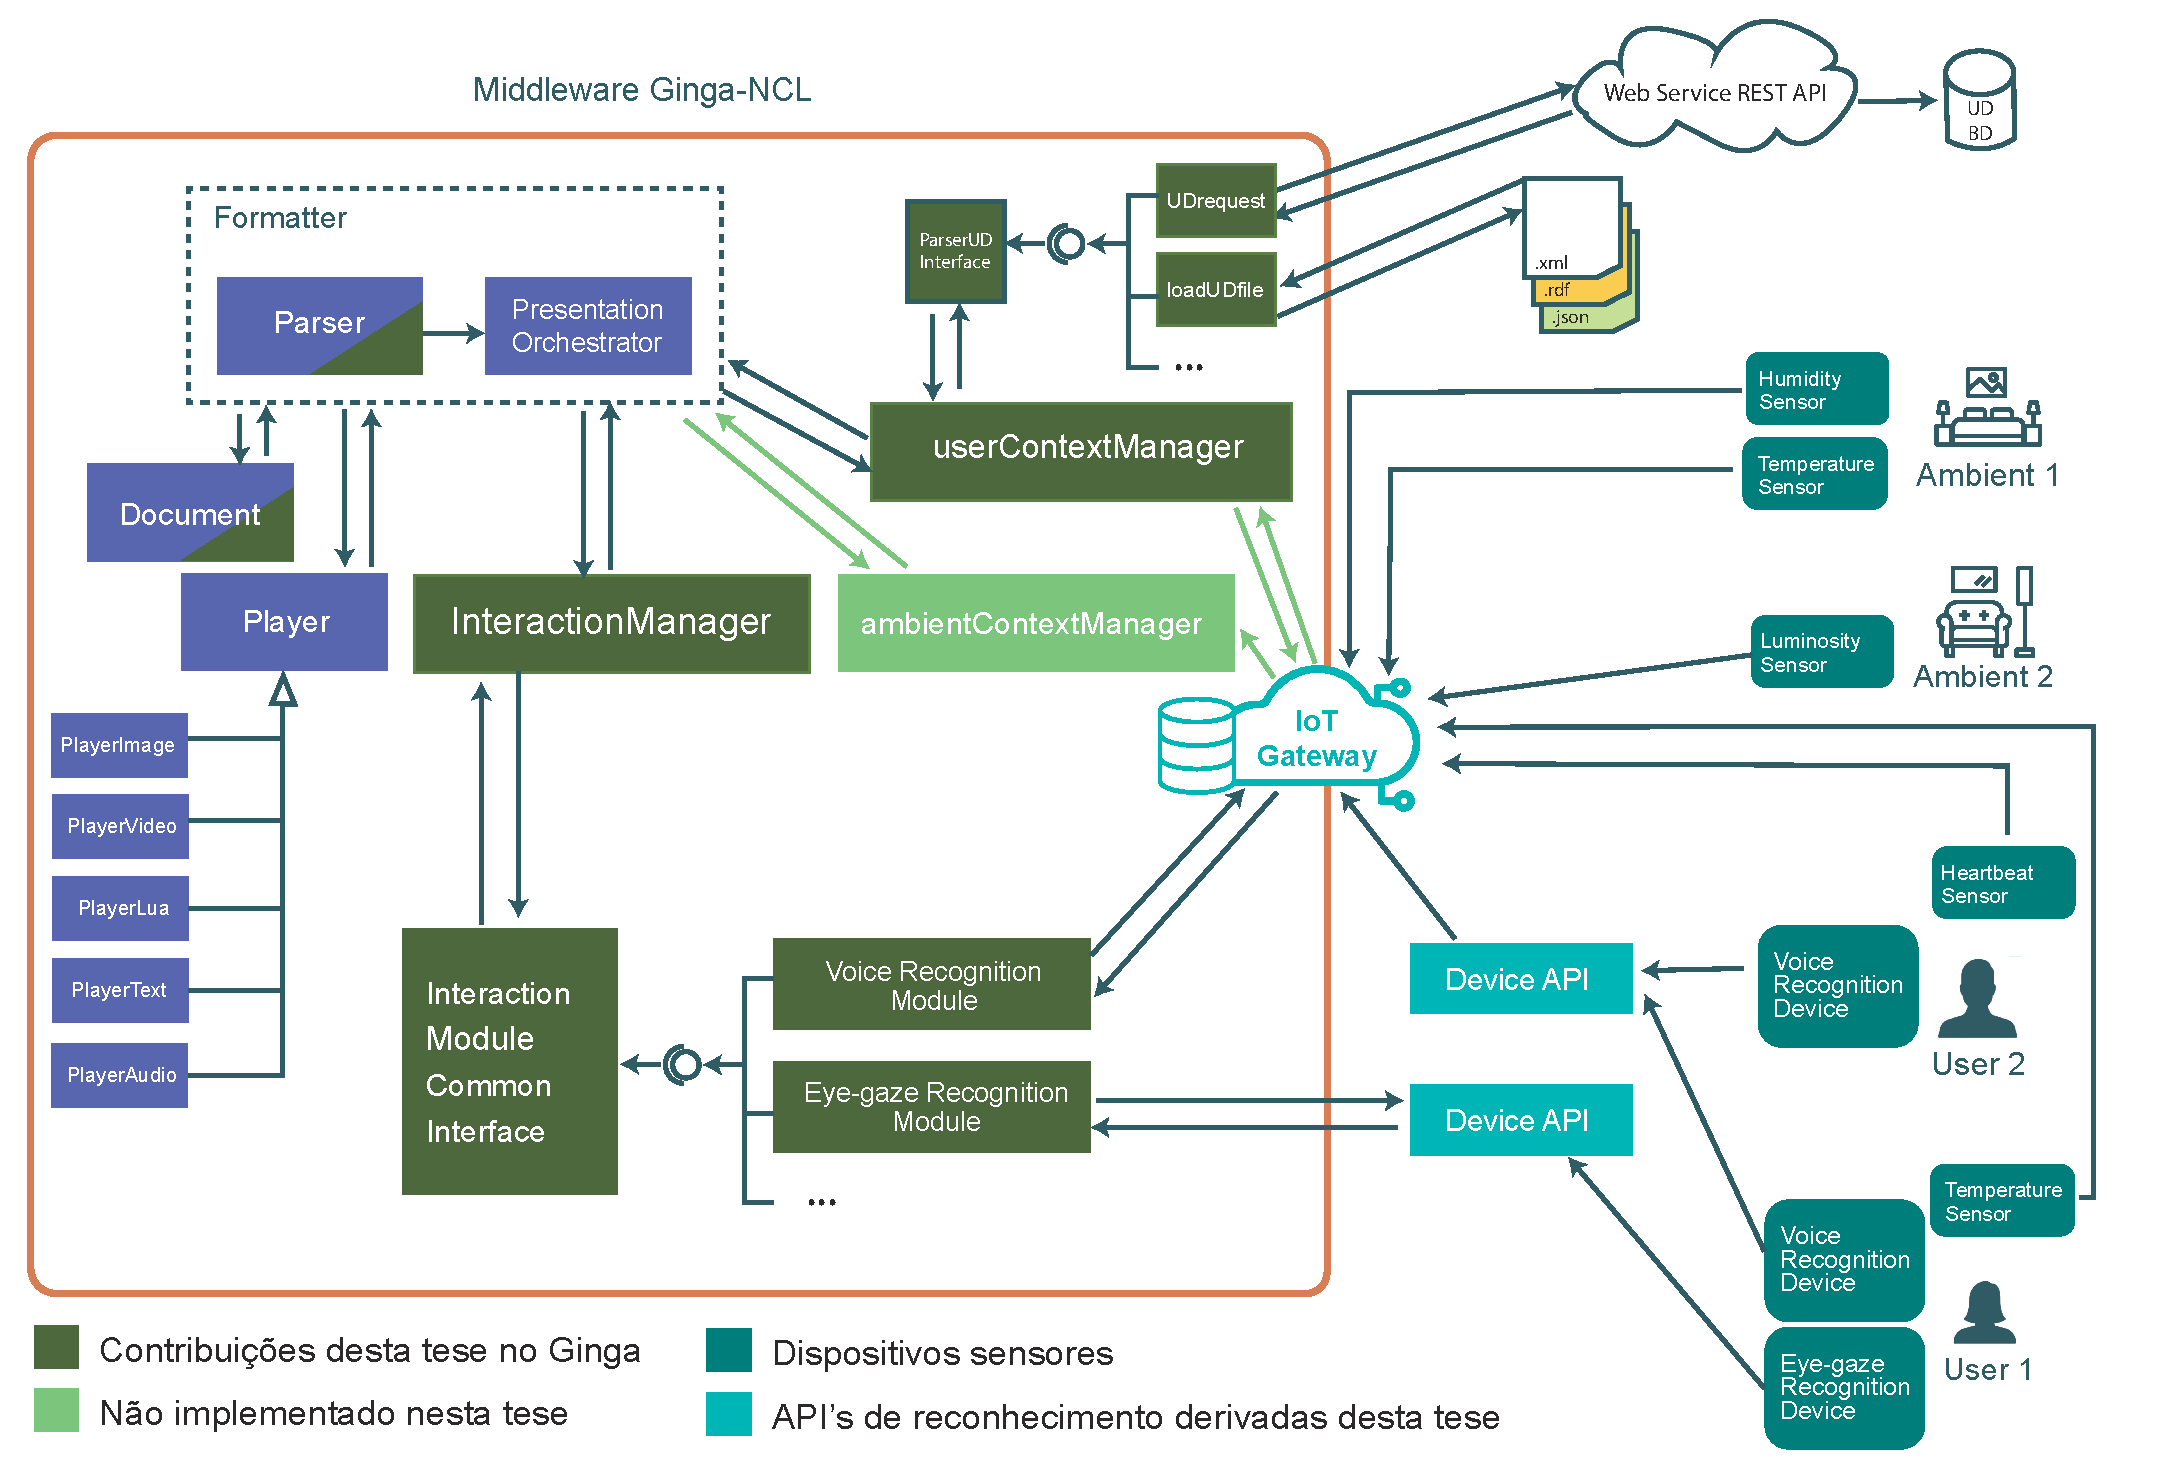
\includegraphics[scale=0.43, keepaspectratio=true]{figuras/ArqPropExt.pdf}
    \caption{Arquitetura estendida do Ginga-NCL para suporte à interação multimodal com múltiplos usuários.}
    \label{fig:arquitetura}
\end{figure}

\section{Interação multimodal e multiusuário}

O componente \textit{Formatter}, presente na atual versão do Ginga, é o responsável por controlar a apresentação dos objetos de mídia que compõem uma aplicação. Além disso, este elemento manipula os eventos de interação do usuário com a aplicação. Ao iniciar uma aplicação multimídia, o \textit{Formatter} envia o documento NCL para o \textit{Parser}, que extrai as informações sobre os elementos que compõem a aplicação e as relações de sincronização espaço-temporal definidas pelo autor da aplicação multimídia. 

O controle das interações do usuário com a aplicação multimídia é realizado pelo componente \textit{InteractionManager} proposto neste trabalho. É por meio do \textit{InteractionManager} que os dispositivos de interação se comunicam com o \textit{Formatter}, notificando-o quando ocorre uma interação por parte do usuário. O \textit{InteractionManager} ativa os diferentes módulos de interação, conforme especificado pelo documento NCL, e passa, para cada um deles, as informações sobre o que deve ser monitorado durante a execução da aplicação. A fim de permitir que a implementação seja facilmente estendida para adição de novas modalidades de interação, foi criada uma interface (\textit{Interaction Module Common Interface}), que deve ser implementada por cada módulo de interação específico. Note que, se a aplicação não utiliza um determinado tipo de interação, o módulo correspondente não será iniciado pelo \textit{InteractionManager} desnecessariamente.

Para a implementação da interação multimodal proposta nesta tese, os componentes \textit{Parser} e \textit{Formatter} foram estendidos, para dar suporte ao reconhecimento de novos tipos de eventos definidos em NCL 4.0 e  detalhados no Capítulo~\ref{cap:cap4}. Se elos da aplicação NCL associam eventos de interação a usuários ou perfis específicos, na fase de análise do documento, o \textit{Parser} faz o mapeamento entre a interação e o usuário associado a ela, por meio da análise dos elementos \textit{<link>} especificados. Por exemplo, ao analisar o elo definido na Listagem \ref{lst:ncl_multmodal}, o \textit{Parser} irá informar ao \textit{Formatter} que é preciso ativar o módulo responsável pelo reconhecimento de voz~(\textit{Voice Recognition Module}), além de enviar para esse módulo o usuário "\textit{user1}" (atributo \textit{user}) e palavra chave  "\textit{play}" (atributo \textit{key}) relacionados à interação e que ele deve notificar ao reconhecedor. Essa notificação é feita ao módulo \textit{InteractionManager}.

\begin{lstlisting}[language=ncl,label=lst:ncl_multmodal, caption={Conector e elo para interação mutimodal em NCL estendido}]

...
<connectorBase>
   <causalConnector id="onVoiceRecognitionStart">
      <connectorParam name="key"/>
      <connectorParam name="user"/>      
      <simpleCondition role="onVoiceRecognition" key="$\$$key" user= "$\$$user"/>
      <simpleAction role="start" />
   </causalConnector>  
</connectorBase>
...
<link xconnector="onVoiceRecognitionStart">
 	<bind role="onVoiceRecognition" component="botanicalGardenImage">
  		<bindParam name="key" value="play"/>
   		<bindParam name="user" value="user1"/>
 	</bind>
 	<bind role="start" component="botanicalGardenVideo"/>
 </link> 
...
\end{lstlisting}

%O controle das interações do usuário com a aplicação multimídia é realizado pelo componente \textit{InteractionManager} proposto neste trabalho. É por meio do \textit{InteractionManager} que os dispositivos de interação se comunicam com o \textit{Formatter}, notificando-o quando ocorre uma interação por parte do usuário. O \textit{InteractionManager} ativa os diferentes módulos de interação, conforme especificado pelo documento NCL, e passa, para cada um deles, as informações sobre o que deve ser monitorado durante a execução da aplicação. A fim de permitir que a implementação seja facilmente estendida para adição de novas modalidades de interação, foi criada uma interface (\textit{Interaction Module Common Interface}), que deve ser implementada por cada módulo de interação específico. Note que, se a aplicação não utiliza um determinado tipo de interação, o módulo correspondente não será iniciado pelo \textit{InteractionManager} desnecessariamente.

Os módulos de interação e o \textit{InteractionManager} se comunicam através de métodos pré-definidos pela interface (\textit{Interaction Module Common Interface}). Por exemplo, o \textit{InteractionManager}, ao ativar um módulo de interação, envia um objeto JSON (\textit{JavaScript Object Notation}) com uma lista de \textit{keys} que devem ser monitoradas pelo módulo, e os usuários relacionados àquela interação. Esta lista de \textit{keys} enviada pelo \textit{InteractionManager} depende do tipo de interação. Por exemplo, para o \textit{Voice Recognition Module}, são enviadas palavras ou frases a serem reconhecidas, e para o \textit{Gesture Recognition Module}, os tipos de gestos utilizados na aplicação. A Listagem~\ref{lst:json-exemplo} mostra um exemplo de JSON que segue o modelo para mapeamento de reconhecimento de voz, que gera o evento definido no \textit{link} na Listagem~\ref{lst:ncl_multmodal}.

\begin{lstlisting}[language=ncl,label=lst:json-exemplo, caption={Exemplo de JSON que usa o modelo para mapeamento de reconhecimento de voz para a Listagem~\ref{lst:ncl_multmodal}.}]
 {
    "userKeyList": [
        {
            "user": "user1",
            "key": [ "play"]
        }
    ]
 }
\end{lstlisting}



Na arquitetura proposta ilustrada na Figura \ref{fig:arquitetura}, pode-se perceber que o trabalho de reconhecimento da interação não é feito pelo formatador, evitando assim uma sobrecarga de processamento. Ele é notificado pelo \textit{InteractionManager} apenas se ocorrer uma interação que deve ser tratada pela aplicação. Ou seja, em uma aplicação multimídia que especifica apenas interação por voz, tendo como \textit{key} a palavra "\textit{play}", caso o usuário diga quaisquer outras palavras diferentes, nenhuma notificação será enviada ao \textit{InteractionManager}, e consequentemente ao formatador. Além disso, quando um módulo de interação específico notifica uma interação, ele pode também informar qual o usuário que a realizou, que no exemplo seria o "user1". Dentre os métodos que os módulos de interação devem implementar estão: \textit{start()}, \textit{setUserKeyList(json)} e \textit{stop()}, que possibilita ao \textit{InteractionManager} iniciar, passar as informações (\textit{keys}) que devem ser reconhecidas e parar o módulo de interação. Estes métodos são virtuais na classe \textit{InteractionModule}, portanto para desenvolver um novo módulo de interação funcionando nesta arquitetura, é necessário estender a classe \textit{InteractionModule}. Exemplos de subclasses de \textit{InteractionModule} na Figura \ref{fig:arquitetura} são \textit{Eye-gaze Recognition Module} e \textit{Voice Recognition Module}. 

\subsection{Reconhecimento de Voz em Ginga-NCL}

Com objetivo de validar a solução proposta, esta seção apresenta a implementação do módulo \textit{VoiceRecognitionModule} no Ginga-NCL utilizando uma API de reconhecimento de voz. A implementação de \textit{VoiceRecognitionModule} no Ginga utiliza a interface de comunicação comum a todos os dispositivos de interação (\textit{Interaction Module Common Interface}). Nesta implementação, o dispositivo de reconhecimento de voz se comunica com o Ginga utilizando o protocolo MQTT \cite{hunkeler2008mqtt}. Para isso, foram usadas funções do \textit{Google Cloud} para suprir a necessidade da conversão \textit{speech-to-text} \cite{bijl2001speech}. Inicialmente, é necessária a aplicação \textit{Google Assistant} para captar a voz do usuário e uma \textit{Action} do Google. Uma \textit{Action} é, essencialmente, uma aplicação que roda sobre o \textit{Google Assistant}, estendendo suas funcionalidades. Como ilustrado pela Figura~\ref{fig:action}, para a \textit{Action} se comunicar com o broker MQTT, ela utiliza o serviço Google \textit{Firebase} para que seja feita a publicação MQTT. 

Em resumo, o \textit{VoiceRecognitionModule} se inscreve em um tópico MQTT criado para o módulo de reconhecimento de voz. Isso é feito na execução do método \textit{start()} e portanto a instância passa a ouvir publicações no tópico que a \textit{Action} usa. Assim, a API do Google publica uma mensagem nesse tópico, significando que o dispositivo reconheceu o que foi dito. Quando ocorre a publicação do texto reconhecido no broker MQTT, o \textit{VoiceRecognitionModule} compara seu conteúdo com a lista de \textit{keys} e \textit{users} de interesse da aplicação. Se for uma palavra ou frase associado a um usuário de interesse ao Ginga, notifica o \texttt{InteractionManager}, que por sua vez dispara o evento de reconhecimento de voz no formatador.

\begin{figure}[h!]
    \centering
    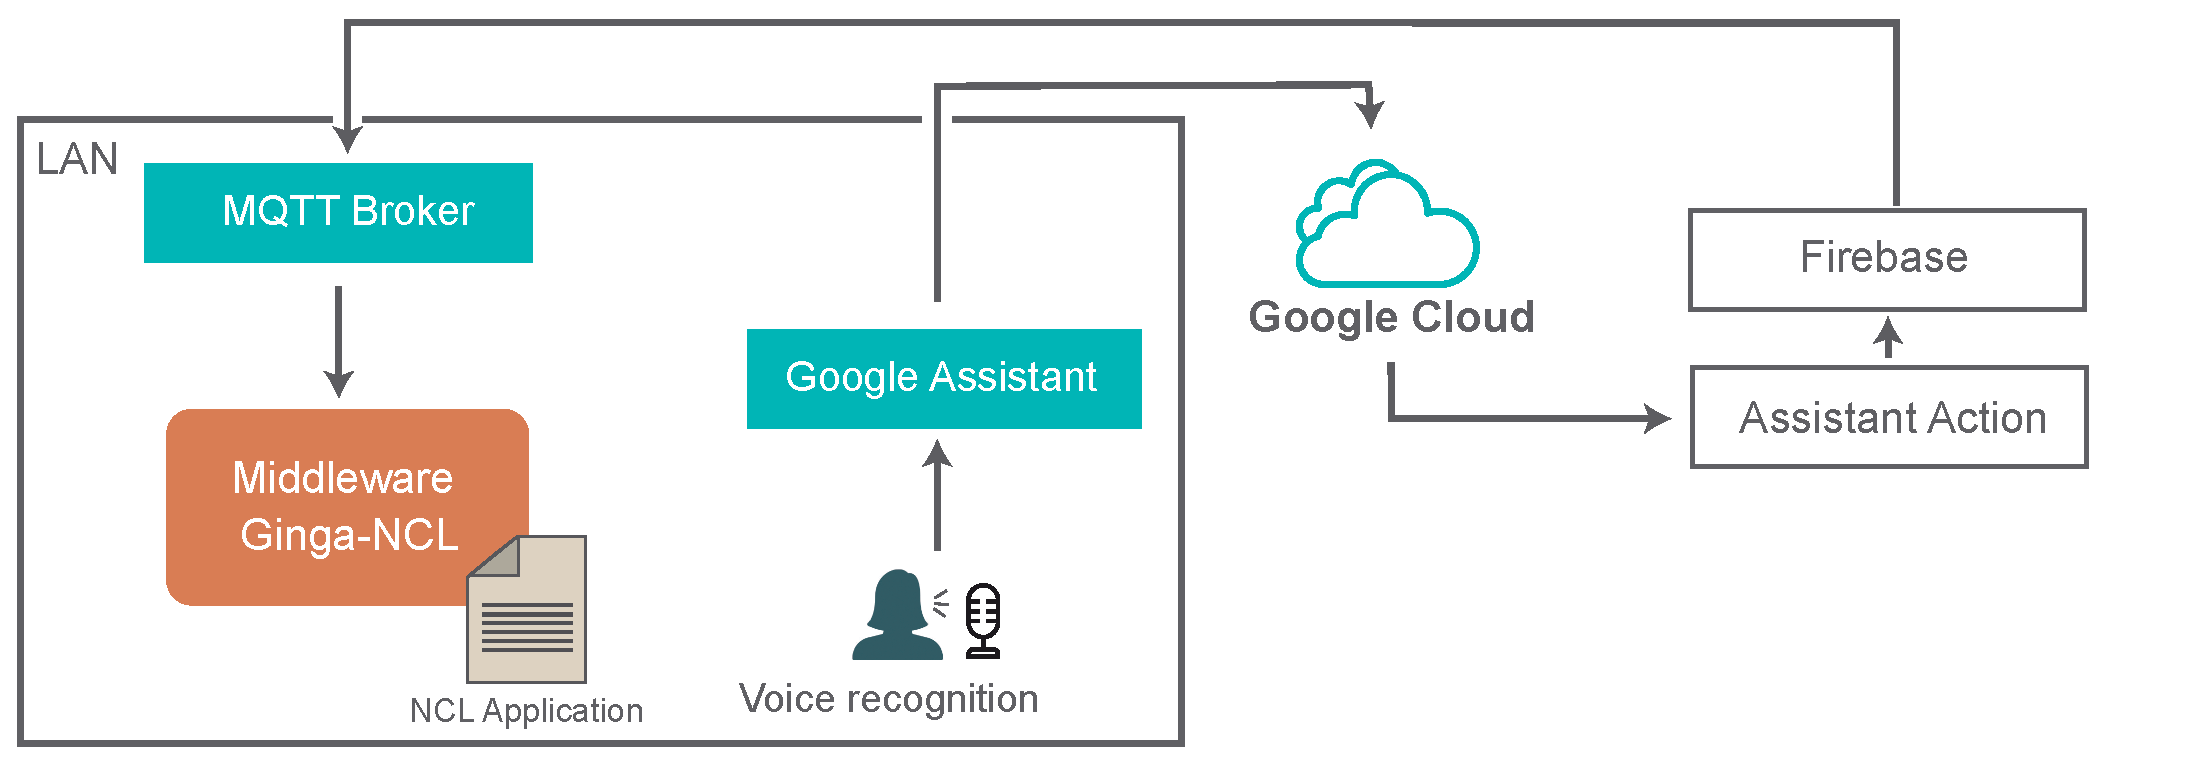
\includegraphics[scale=0.35, keepaspectratio=true]{figuras/arq-action-eng.pdf}
    \caption{Arquitetura do reconhecimento de voz na implementação atual.}
    \label{fig:action}
\end{figure}

A \textit{Action}, ao ser invocada, encaminha em forma de texto, todos comandos de voz que sejam precedidos por "TV". Desse modo, caso se queira executar na aplicação um comando denominado "iniciar", diz-se "TV iniciar". Há, ainda, uma configuração opcional de perfis de usuário. Ao dizer "Definir perfil como...", o que vier depois é vinculado ao dispositivo corrente como sendo o perfil ou a identificação daquele usuário. Feito isso, todos os comandos enviados à aplicação são precedidos por esse perfil ou identificação, relacionado ao usuário que interagiu.

A título de exemplo, em uma aplicação que contém um terapeuta e um paciente, de forma que cada perfil tem acesso a um conjunto de comandos diferentes, o usuário ao se identificar por terapeuta, em seu dispositivo, invoca "Definir perfil como terapeuta" e, analogamente, o paciente faz o mesmo. A partir disso, a aplicação será capaz de decidir, baseado nos perfis, quem invoca qual comando.

Outra implementação, seguindo a arquitetura da Figura~\ref{fig:arquitetura}, foi proposta em \cite{montevecchi2020providing}, onde sensores de rastreamento ocular permitem que os usuários interajam pelo olhar com aplicativos multimídia, proporcionando assim também uma nova modalidade de interação para as aplicações de TV digital. Em \cite{montevecchi2020providing}, foi proposta uma extensão Ginga-NCL para fornecer interação através de fixação do olhar usando um dispositivo rastreador de olhos e permitir o uso de um novo tipo de evento para autoria  em NCL, chamado \textit{EyeGaze}.

O trabalho de  \cite{valentim2020possibilitando} utiliza a  arquitetura proposta na Figura~\ref{fig:arquitetura} para possibilitar o reconhecimento de expressões faciais para que a TV que seja agnóstica à implementação do algoritmo de reconhecimento. Como prova de conceito, a  proposta do artigo foi desenvolvida sob o \textit{middleware} Ginga-NCL. Foram realizadas duas implementações: a primeira baseada na versão atual do \textit{middleware} Ginga e a segunda baseada em uma extensão proposta ao \textit{middleware}, mostrando a viabilidade da proposta apresentada.

\section{Suporte Multiusuário e Informações de Contexto}

A atual versão do \textit{middleware} Ginga-NCL captura as interações vindas de dispositivos como controle remoto, mouse ou teclado representando a interação de um usuário somente. Suas informações são armazenadas em um nó de conteúdo do tipo \textit{settingsNode} onde também são armazenadas informações gerais da aplicação NCL. Só é permitido um nó desse tipo por aplicação NCL. Algumas dessas propriedades não podem ser alteradas durante a execução da aplicação. Se mais de um usuário interage com a aplicação e essa precisa mudar seu comportamento de acordo com propriedades específicas de quem participa da experiência, não seria possível construir um documento NCL para atender a esse caso de uso na versão atual do Ginga-NCL.

O elemento XML <\textit{userAgent}> foi implementado por meio de uma estrutura \textit{user} que armazena propriedades de um usuário como um identificador e o caminho do arquivo onde estão suas informações individuais. Já o <\textit{userProfile}> foi implementado com a construção da estrutura \textit{profile} que mantém um identificador, numero mínimo e máximo de usuários que podem estar associados ao perfil e o caminho para as informações do perfil. A implementação mantém, no formatador, uma lista de estruturas do tipo \textit{user} e outra lista do tipo \textit{profile}. Desta forma, é possível ao formatador associar os \textit{links} de interação com os usuários ou perfis a estas listas; Carregar informações destes usuários para nós de conteúdo do tipo \textit{userSettingsNode} podendo também criar elos com esses nós. Finalmente pode-se associar a essa lista sensores, que podem coletar informações dos usuários participantes da experiência multimídia, como batimento cardíaco ou temperatura.

Os elos são associados ao usuário da maneira como foi descrita na Seção anterior, ou seja, o \textit{InteractionManager} envia para os módulos as listas de usuário que participam dos elos por meio de seu atributo \textit{user}. O valor do atributo \textit{user} deve fazer parte das listas de \textit{users} ou \textit{profiles} mantidas pelo formatador. Assim o autor da aplicação precisa definir o elemento  \textit{userAgent} e/ou \textit{userProfile} para poder referenciá-lo em elos com eventos de interação.

Conforme apresentado na Figura~\ref{fig:arquitetura}, o \textit{userContextManager} gerencia a importação das informações associadas tanto a \textit{userAgent} quanto a \textit{userProfile}. As informações podem estar dispostas em arquivos como por exemplo XML, RDF ou JSON ou ainda estarem disponíveis em um banco de dados remoto  acessado por meio de API REST. O caminho do arquivo ou a string de conexão fica armazenada no atributo \textit{src} do \textit{userAgent} ou \textit{userProfile}. O carregamento dessas informações é feito por um módulo que implementa a interface \textit{ParserUDInterface}, como por exemplo, \textit{UDRequest} e \textit{loadUDFile}. Este módulo irá carregar todas as informações presentes no arquivo ou no banco de dados de acordo com a fonte de cada um. Para que um novo formato de arquivo seja contemplado pelo \textit{userContextManager}, basta implementar um classe filha de \textit{ParserUDInterface}. O módulo \textit{userContextManager} irá passar aos "importadores" (módulos que implementam \textit{ParserUDInterface}) todos os dados necessários para importação e armazenamento das propriedades desses usuários ou perfis. 

As informações trazidas serão armazenadas em nós de conteúdo do tipo \textit{userSettingsNode} gerenciados pelo \textit{UserContextManager}. Esses nós são instâncias de \textit{userSettingsNode} associados aos elementos  <\textit{userAgent}> ou <\textit{userProfile}>. Como prova de conceito, foi desenvolvido o módulo \textit{loadUDFile} para  arquivos XML seguindo o padrão MPEG-21 parte 22. Este módulo vai preencher o objeto da classe \textit{UserSettingsNode} associado a instância do \textit{UserAgent} respectivo.  Se o \textit{UserAgent} estiver associado ao \textit{UserProfile}, além das informações individuais referenciadas no \textit{UserAgent}, também serão consideradas as informações associadas aos \textit{UserProfiles}. A partir do momento em que as informações estão em nós do tipo \textit{userSettingsNode}, poderão ser utilizadas em elos com eventos de atribuição NCL.

As instâncias de \textit{UserSettingsNode} podem ser usadas também para armazenar informações lidas de um sensor em um ambiente IoT. Como pode-se verificar na Figura~\ref{fig:arquitetura}, pode-se ter sensores (com por exemplo \textit{Heartbeat Sensor} no User2) publicando leituras em um servidor IoT e o \textit{userContextManager} pode ler essas publicações e atualizar os nós do tipo \textit{UserSettingsNode} respectivos. Para isso, o gerenciador de contexto deve ter um assinante de um tópico no servidor IoT. Tomando como exemplo a arquitetura MQTT, pode-se ter um \textit{broker} MQTT recebendo publicações dos sensores e o gerenciador de contexto pode se inscrever nos mesmos tópicos de publicações dos sensores e atualizar as propriedades respectivas nos nós de conteúdo do tipo \textit{userSettingsNode} a partir da atualização das propriedades. Elos poderão ser ativados mudando o comportamento da aplicação de acordo com leituras feitas pelos sensores. De maneira análoga, o mesmo pode ser feito com sensores de ambiente (como por exemplo \textit{LuminositySensor} no Ambient 2 na Figura~\ref{fig:arquitetura}), publicando suas leituras no servidor IoT. E o gerenciador de contexto de ambientes (\textit{ambientContextManager}) pode pegar essas informações e atualizar os nós do tipo \textit{ambientSettingsNode}. Como também são nós de conteúdo, a atualização de suas propriedades pode ativar elos e disparar ações na aplicação. A implementação do \textit{ambientContextManager} 
é trabalho futuro.

Além de ler as informações publicadas pelos sensores de um servidor IoT, O \textit{userContextManager} pode também publicar informações específicas para que o dispositivo IoT leia, como por exemplo, informações para calibragem do dispositivo. Assim o gerenciador pode-se comunicar com o servidor nos dois sentidos. A comunicação entre o \textit{userContextManager} e o servidor IoT também 
é trabalho futuro.

Falta ressaltar que a arquitetura é extensível a vários tipos de evento de interação, dispositivos e sensores.

Este capítulo apresentou a implementação da proposta desta tese no \textit{middleware} Ginga-NCL, incluindo uma arquitetura extensível seus módulos e funcionamento geral. O capítulo exemplificou aplicações NCL desenvolvidas e utilizadas nos testes de funcionalidades. Apresentou também o formato dos dados que são trocados entre os módulos, como por exemplo, objetos JSON. O próximo capítulo apresenta a avaliação da proposta por meio de comparação com a implementação padrão atual do Ginga-NCL e também testes de carga que atestam o desempenho do \textit{middleware}.
\chapter{Avaliação} \label{cap:cap6}

Este capitulo apresenta várias abordagens utilizadas para avaliar a proposta desta tese. Primeiramente, a Seção~\ref{sec:CompNCL30} apresenta a execução de experimentos para avaliar como a extensão proposta se comporta em comparação a uma implementação do reconhecimento de voz usando o Ginga-NCL padrão atual com scripts Lua. A Seção~\ref{sec:cargaNCL40} apresenta a realização de um teste de carga da capacidade de manipulação de eventos do \textit{middleware}, tratando vários eventos multimodais em diversos intervalos de tempo. A Seção~\ref{sec:performanceNCL40} apresenta os testes para avaliar se houve perda de desempenho no \textit{middleware} no tratamento do eventos sendo disparados em vários intervalos de tempo de disparos, assim como intervalos de tempo diferentes para acordar os processos de leitura do servidor MQTT. Ja na Seção~\ref{sec:cargaUsuariosNCL40} apresenta a avaliação se o tratamento de perfil de multiusuários causa algum atraso significativo ao \textit{middleware}.  Além da abordagem avaliativa, este capitulo apresenta uma seção de casos de uso onde as novas funcionalidades se fazem necessárias, alguns desses casos de uso foram implementados e executados na nova versão do \textit{middleware}.

\section{Multimodalidade}\label{sec:AvMultimodalidade}

As subseções seguintes apresentam avaliação da multimodalidade, os seja, uma análise quantitativa de como o tratamento de evento de interação multimodal esta sendo realizado pelo \textit{middleware}.

\subsection{Avaliação comparativa} \label{sec:CompNCL30}

Este seção apresenta um cenário de uso para destacar como NCL estendida suporta o desenvolvimento de uma aplicação multimídia com interação de voz por múltiplos usuários. Para tal, a seção descreve uma aplicação NCL que tem como objetivo representar um cenário em que o usuário "\textit{UO1}" controla um vídeo que faz um \textit{tour} pelo Jardim Botânico. Desta maneira, apenas o usuário "\textit{U01}" pode manipular a apresentação do vídeo. Para demonstrar a implementação do evento de voz, foi desenvolvida um aplicação que inicia um vídeo a partir do comando de "\textit{play}" dito pelo usuário "\textit{U01}". As Listagens \ref{lst:ncl_multmodalNCL30} e \ref{lst:ncl_multmodal_} apresentam o conector e o link relacionado com o início do vídeo do Jardim Botânico, ativado por comando de voz. Escritas em NCL 3.0 e NCL 4.0 respectivamente.

O exemplo da Listagem~\ref{lst:ncl_multmodalNCL30} utiliza um evento de reconhecimento de voz (\textit{voiceRecognition}) por meio do script \textit{scriptInt.lua} (linha 16), que o autor precisa desenvolver e iniciá-lo junto com a aplicação que neste caso foi feita por meio do link da linha 20. Além disso será necessário um conector do tipo \textit{onEndAttribution} com um \textit{compoudCondition} para o teste que verificará se uma \textit{string} contém a palavra que indica que o "\textit{U01}" disse "play".

\begin{lstlisting}[language=ncl,label=lst:ncl_multmodalNCL30, caption={Conector e elo para interação mutimodal em NCL 3.0}]
...
<connectorBase>
  <causalConnector id="onEndAttributionTestStart">    	
    <connectorParam name="val"/>
      <compoundCondition operator="and">
        <simpleCondition role="onEndAttribution"/>       	
	    <assessmentStatement comparator="eq">
	      <attributeAssessment role="attNodeTest" eventType="attribution" attributeType="nodeProperty"/>
	      <valueAssessment value="$\$$val"/>
	    </assessmentStatement>
	  </compoundCondition>
   	  <simpleAction role="start"/>
  </causalConnector>
</connectorBase>
...
<media id="readIntModes" src="scripts/scriptInt.lua">
  <property name="key"/> 
</media>
...
<link xconnector="onBeginStart">
  <bind role="onBegin" component="botanicalGardenImage"/>
  <bind role="start" component="readIntModes" />
</link>
<link xconnector="onEndAttributionTestStart">
  <bind role="onEndAttribution" component="readIntModes" interface = "key"/>
  <bind role="attNodeTest" component="readIntModes" interface="key">
	<bindParam name="val" value="voice_recog/U01:play"/>
  </bind>	
  <bind role="start" component="botanicalGardenVideo"/>
</link>
...
\end{lstlisting}

O exemplo da Listagem~\ref{lst:ncl_multmodal_} utiliza um evento de reconhecimento de voz (\textit{voiceRecognition}) por meio do papel pré-definido \textit{onVoiceRecognition}. Esta condição possui um atributo \textit{key} que identifica o palavra a ser captada. Ainda, o atributo \textit{user} indica que tal palavra deverá ser captada do usuário (\textit{U01}).

\begin{lstlisting}[language=ncl,label=lst:ncl_multmodal_, caption={Conector e elo para interação mutimodal em NCL estendido}]
...
<connectorBase>
   <causalConnector id="onVoiceRecognitionStart">
      <connectorParam name="key"/>
      <connectorParam name="user"/>      
      <simpleCondition role="onVoiceRecognition" key="$\$$key" user= "$\$$user"/>
      <simpleAction role="start" />
   </causalConnector>  
</connectorBase>
...
<link xconnector="onVoiceRecognitionStart">
 	<bind role="onVoiceRecognition" component="botanicalGardenImage">
  		<bindParam name="key" value="play"/>
   		<bindParam name="user" value="U01"/>
 	</bind>
 	<bind role="start" component="botanicalGardenVideo"/>
 </link> 
...
\end{lstlisting}

Para avaliar a o comportamento do evento \textit{VoiceRecognition} na extensão proposta, foram construídas três aplicações NCL derivadas do exemplo na Listagem~\ref{lst:ncl_multmodal_} \footnote{As aplicações NCL e o \textit{script} de testes podem ser acessados em http://bit.do/fHiw4}. A primeira aplicação inicia um vídeo quando for dito "\textit{play}" pelo usuário "U01". A segunda aplicação inicia automaticamente um vídeo e para este vídeo, quando for dito "\textit{stop}" pelo usuário "U01". A terceira aplicação inicia automaticamente um vídeo e pausa o vídeo, quando for dito "\textit{pause}" pelo usuário "U01". 

As aplicações foram desenvolvidas em duas versões. Primeiro na versão em NCL 4.0 proposta neste trabalho. Para executá-la, foi utilizada a versão Ginga-NCL 4.0 apresentada no Capítulo~\ref{cap:cap5}. A segunda versão das aplicações foi construída utilizando NCL 3.0 e scripts NCLua emulando o comportamento do evento \textit{VoiceRecognition}.

Em todos os testes, a forma de disparar o evento de interação por voz foi simplificada para que o teste não fosse comprometido com o retardo de reconhecimento da API na nuvem da Google. Desta forma, foi produzido um script que inicia a aplicação e publica um texto no tópico \textit{voiceRecognition} de um \textit{broker} MQTT rodando na mesma máquina que o \textit{middleware} Ginga. A publicação no tópico \textit{voiceRecognition} sinaliza que algo foi dito.

Após a publicação no tópico, o \textit{VoiceRecognitionModule} deve perceber uma atualização no tópico. A partir deste momento, na versão 4.0 da classe implementada seguindo a arquitetura apresentada no Capítulo~\ref{cap:cap5} notifica o formatador sobre o evento de reconhecimento de voz. 

Na versão das aplicações em NCL 3.0, foi implementado um script NCLua que acessa o tópico MQTT desejado e dispara um evento de atribuição na aplicação NCL, que por sua vez possui links para sincronizar a atribuição com uma ação no vídeo.

Cada aplicação foi construída para testar e medir o tempo gasto desde o reconhecimento de voz até o inicio de alguma de três ações ("start", "stop" e "pause"). Experimentos foram executados com cada uma das aplicações a fim de avaliar e comparar o tempo de resposta da proposta de NCL 4.0 e de uma aplicação NCL 3.0 com \textit{scripts} Lua. Os resultados foram obtidos de uma média de 100 execuções. Os experimentos foram realizados em uma máquina com as seguintes configurações: Intel$^{\tiny{\textregistered}}$ Core™ i5-7500T CPU @ 2.70GHz; 8GB RAM; 1TB HD e Sistema Operacional Ubuntu 18.

O tempo médio ($T$) calculado em cada  experimento é definido por: 
\[ T = \sum_{i=1}^{100}{\frac{mqttPub_i+responseTime_i}{100}}\]

Onde $mqttPub$ é o tempo de comunicação entre a postagem de dados no tópico do broker, o processamento do \textit{broker} e a percepção de atualização deste tópico pelo cliente MQTT. $responseTime$ é o tempo que o Ginga demora para executar a ação esperada a partir do momento em que é reconhecida a publicação no tópico MQTT.

Na Figura~\ref{fig:grafAvaliacao}, são apresentados os resultados de experimentos para as três aplicações em suas duas versões com intervalo de confiança de 95\%. Na cor azul, é apresentado o tempo médio das aplicações criadas com NCL 4.0. Na cor verde, pode-se observar o tempo médio das aplicações criadas com NCL 3.0 e scripts NCLua. Pode-se observar que a aplicação com a proposta deste trabalho com NCL 4.0 possui tempo de resposta abaixo de 70$ms$ enquanto todas as aplicações feitas em NCL 3.0 superam 200$ms$ para responder a ação. 

\begin{figure}[h!]
    \centering
    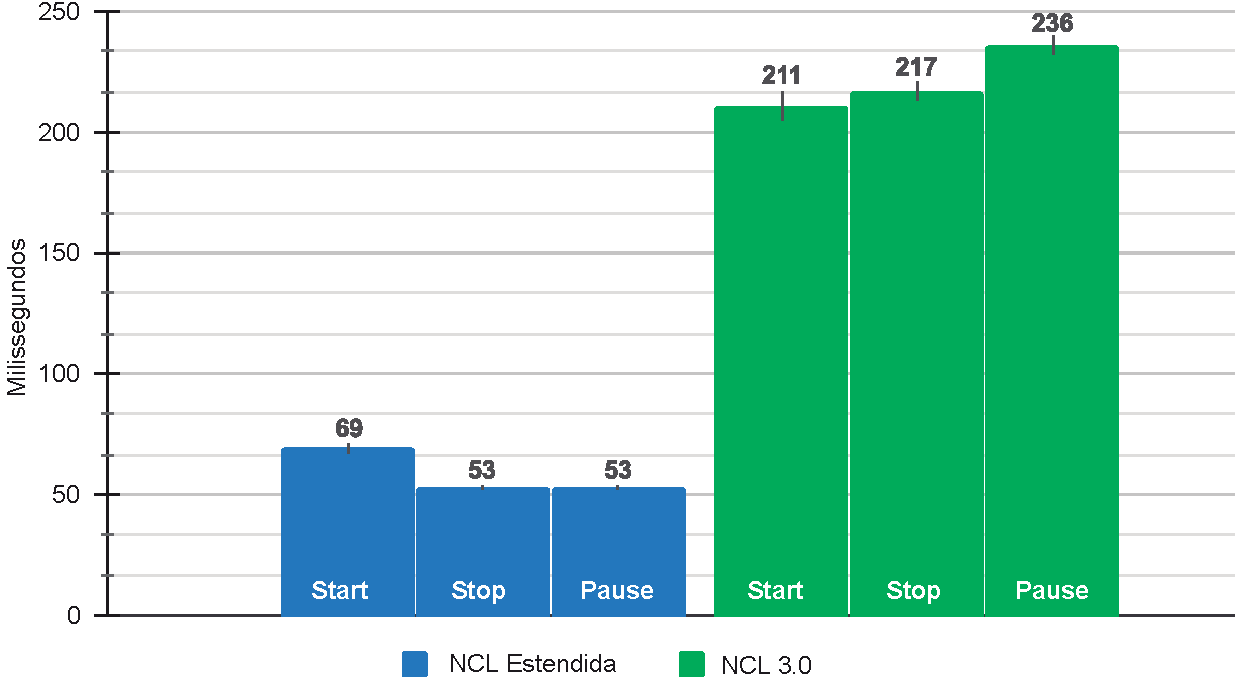
\includegraphics[scale=0.5, keepaspectratio=true]{figuras/graficoAvaliacao1.pdf}
    \caption{Média de tempo (ms) gasto para aplicação reagir a uma publicação MQTT de start/stop/pause em uma mídia.}
    \label{fig:grafAvaliacao}
\end{figure}

Como pode ser visto na Figura~\ref{fig:grafAvaliacao}, o tempo de resposta de uma aplicação em NCL 4.0 é aproximadamente um terço do tempo de uma aplicação feita utilizando NCL 3.0 e Lua. Além disso, em NCL 4.0, o autor da aplicação não precisa programar em uma linguagem imperativa e não precisa acoplar módulos ou scripts NCLua à sua aplicação existente. Estes resultados demonstram que a implementação de interação multimodal proposta no Ginga oferece bom desempenho.

Com o uso de NCL 4.0, também há uma diminuição do esforço de autoria. O autor da aplicação, usando NCL 4.0, deve declarar apenas $1$ conector e $1$ link para prover a interação por voz. A aplicação tem um total de $49$ linhas de código para descrever seu comportamento. Por outro lado, em NCL 3.0, o autor necessita de scripts NCLua para realizar o acesso aos tópicos MQTT e criação de um conector de atribuição para emular um evento de reconhecimento de voz. A aplicação NCL 3.0 tem um total de $158$ linhas de código.

Adicionalmente, a forma de descrever interação multimodal por meio de eventos da linguagem NCL favorece a legibilidade do código NCL. Pois quando o usuário define um conector com o papel \textit{onVoiceRecognition}, é mais fácil de entender que se trata de um reconhecimento de voz do que ter que criar um conector com papel  \textit{onEndAtribution} para tratar o evento de reconhecimento de voz gerado pelo \textit{script} Lua.

\subsection{Avaliação de carga} \label{sec:cargaNCL40}

Para avaliar a capacidade do \textit{middleware} de lidar com inúmeros eventos multimodais, esta seção apresenta vários testes realizados que usaram várias aplicações NCL simples. Essas aplicações possuíam links que eram disparados com eventos de interação por meio de voz e gesto. As interações foram representadas no teste por meio de publicações em tópicos MQTT onde os dispositivos responsáveis por essas interações multimodais publicam. Isso foi possível por causa da execução de um \textit{script} fazendo as publicações. O \textit{middleware} ouviu  esses tópicos por meio dos módulos de interação (IMs). Sempre que ocorreu uma publicação, os IMs sinalizaram para o \textit{middleware}, que por sua vez sinalizou para todos objetos interessados nos eventos na aplicação NCL. Assim, o teste utilizou uma aplicação NCL que alterava uma variável cada vez que uma publicação era recebida, ou seja, para confirmar que a ação aconteceu e que o evento foi capturado. Para avaliar esse comportamento, a aplicação foi executada com os módulos do \textit{middleware} ouvindo eventos a cada 10 milissegundos. Este é um parâmetro do Ginga que pode ser configurado. O teste emulou 100 eventos disparados em intervalos de 10$ms$; 15$ms$; 20$ms$; 30$ms$; 40$ms$ e 50$ms$ e contou quantos eventos foram capturados e manipulados para cada valor de intervalo. O teste repetiu esse processo 100 vezes e, em seguida, calculamos a média de cada intervalo. A Figura~\ref{fig:grafAvaliacao2} mostra os resultados obtidos. Podemos ver que, para os intervalos de 20$ms$ e superiores, o Ginga obteve uma excelente taxa de captura de eventos, atingindo em média 99,9\% de capturas.
\begin{figure}[h!]
    \centering
    \includegraphics[scale=0.50, keepaspectratio=true]{figuras/grafEventosCap.pdf}
    \caption{Média do número de eventos capturados}
    \label{fig:grafAvaliacao2}
\end{figure}


\subsection{Avaliação de performance} \label{sec:performanceNCL40}

Neste experimento, o teste avalia o quanto esse tratamento de novos eventos retarda a extensão do \textit{middleware} proposta. Para isso, primeiramente o teste mediu o atraso causado pela escuta dos módulos sem acionar os eventos e depois ouvindo o acionamento do evento. O teste utilizou \textit{scripts} que realizaram essas publicações MQTT em intervalos de 20\textit{ms}, que é o menor intervalo com 99,9\% dos eventos capturados, conforme encontrado na Figura~\ref{fig:grafAvaliacao2}. Para isso, uma aplicação NCL foi criada com uma imagem de fundo com âncoras temporais que iniciaram quatro outras imagens. Para cada segundo, uma nova imagem foi iniciada. A visão temporal deste aplicativo é mostrada na Figura~\ref{fig:timeView}. A aplicação foi executada 100 vezes, e o teste calculou a média do tempo de início de cada imagem associada às âncoras temporais. Essas execuções foram feitas em três cenários diferentes: 

             (1) Rodar a aplicação sem os IMs (Ginga-NCL estendido sem iniciar os IMs);
             
             (2) Rodar a aplicação com os IMs sem receber eventos de interação (IMs iniciados com Ginga-NCL estendido);
             
             (3) Executar a aplicação com os IMs e receber 300 eventos de interação (150 eventos de reconhecimento de voz e 150 gestos) (Ginga-NCL estendido iniciando e sobrecarregando IMs).

\begin{figure}[h!]
    \centering
    \includegraphics[scale=0.50, keepaspectratio=true]{figuras/VisaoTemporalAppCarga.pdf}
    \caption{Visão Temporal da aplicação usada para avaliar o atraso em três diferentes cenários}
    \label{fig:timeView}
\end{figure}

A Figura~\ref{fig:average} mostra o atraso médio da apresentação de cada objeto de mídia nesses três cenários diferentes. Observe que nos cenários (2) e (3), o \textit{middleware} desperta o ouvinte a cada 10$ms$. No cenário (2), podemos observar que o ouvinte, sem disparar os eventos causa um atraso da ordem de 9$ms$. No cenário (3), o disparo de 300 eventos no intervalo de 20$ms$, com os módulos acordando e ouvindo a cada 10$ms$.
Podemos ver na Figura~\ref{fig:average} que a extensão proposta não impacta o \textit{middleware} Ginga quando nenhum ouvinte de evento multimodal está ativo. Além disso, para o cenário (2) o atraso médio resultante foi de $\approx$ 6$ms$ e para o cenário (3) o atraso médio foi de $\approx$ 11$ms$. A implementação de nossos ouvintes adiciona pelo menos um atraso de $\approx$ 6$ms$ na implementação estendida do Ginga-NCL; no entanto, esse atraso não aumenta à medida que o número de eventos aumenta. Além disso, o pior caso de atraso no cenário (3) foi de 13$ms$ em \textit{img1}. De acordo com o trabalho de Card et. al \cite{card1986model}, leva 230 $ms$ para um humano perceber algo visualmente. Assim, como nosso pior cenário adiciona à percepção de \textit{img1} um atraso de $\approx \frac{1}{17}$ do tempo identificado em \cite{card1986model}, ele não representa um impacto na apresentação de \textit{img1}.

\begin{figure}[h!]
    \centering
    \includegraphics[scale=0.60, keepaspectratio=true]{figuras/scenarios.pdf}
    \caption{Média de atraso (em ms) de cada mídia na aplicação para cada cenário}
    \label{fig:average}
\end{figure}


\section{Multiusuário}\label{sec:AvMultiusuario}

Esta seção apresenta avaliação de multiusuário, ou seja, uma análise quantitativa de como \textit{middleware} se comporta com o tratamento das funcionalidades para uma aplicação multiusuário especificadas neste trabalho. Para isso, esta seção apresenta a avaliação em duas partes. A primeira mede tempo gasto no reconhecimento dos usuários cujo propriedades estão armazenadas em arquivos XML. A maior processamento acontece quando a aplicação tem um perfil a ser validado. Pois conforme foi dito no Capitulo~\ref{cap:cap4}, quando a aplicação tem algum \textit{userProfile}, todas as propriedades são comparadas com as propriedades de todos os usuários que estão armazenados no \textit{setbox}. Assim, somente os usuários que tenha tais propriedades, irão ter suas interações consideradas pelo \textit{middleware}. A segunda parte mede o tempo gasto para criação de todos o links dinâmicos a partir dos usuários encontrados e que atendam o perfil.

Os resultados foram obtidos de uma média de 100 execuções. Os experimentos foram realizados em uma máquina com as seguintes configurações: Intel$^{\tiny{\textregistered}}$ Core™ i5-7500T CPU @ 2.70GHz; 8GB RAM; 1TB HD e Sistema Operacional Ubuntu 18.

Na primeira parte cada aplicação foi construída para testar e medir o tempo gasto para reconhecer de todos os usuários com o perfil especificado na aplicação. Para isso, o experimento usou 5 cenários onde varia o número de usuários e de propriedades comparadas com as propriedades do perfil usado. A Tabela~\ref{tab:expUserPerfil} apresenta os cenários com a média dos tempos gasto para carregar os usuários em 100 execuções.

\begin{table}[h]
\centering
{
  % distancia entre a linha e o texto
  \renewcommand\arraystretch{1.25}
  \begin{tabular}{|p{1,5cm}|p{6cm}|p{1,5cm}|p{2cm}|} \hline
   \multicolumn{1}{|c|}{Cenário} & \multicolumn{1}{|c|}{Descrição} & \multicolumn{1}{c|}{Média (ms)} & \multicolumn{1}{c|}{Confiança} \\\hline
    1 & 1 usuário com 5 propriedades &  0  & 1,09E-09    \\\hline
    2 & 5 usuários com 5 propriedades &  1  & 2,04E-09   \\\hline
    3 & 10 usuários com 5 propriedades &  1  & 7,76E-10  \\\hline
    4 & 5 usuários com 10 propriedades &  1  & 1,06E-09  \\\hline
    5 & 10 usuários com 10 propriedades &  1  & 1,47E-09 \\\hline
   \end{tabular}
\caption{Cenários contemplados no experimento para usuários de um perfil}
\label{tab:expUserPerfil}
}
\end{table}

Na segunda parte cada aplicação foi construída para testar e medir o tempo gasto para criar os links dinâmicos para cada usuário. Para isso, o experimento usou 9 cenários onde varia o número de usuários e de links com perfil usado. A Tabela~\ref{tab:expUserPerfil} apresenta os cenários com a média dos tempos gasto para carregar os usuários em 100 execuções.

\begin{table}[h]
\centering
{
  % distancia entre a linha e o texto
  \renewcommand\arraystretch{1.25}
  \begin{tabular}{|p{1,5cm}|p{6cm}|p{1,5cm}|p{2cm}|} \hline
   \multicolumn{1}{|c|}{Cenário} & \multicolumn{1}{|c|}{Descrição} & \multicolumn{1}{c|}{Média (ms)} & \multicolumn{1}{c|}{Confiança} \\\hline
   
   1 & 1 link com 1 user & 0 & 0 \\\hline
   2 & 10 links com 1 user & 0 & 5,89E-10 \\\hline
   3 & 50 links com 1 user & 0 & 9,40E-10 \\\hline	 	
   
   4 & 1 link com 5 users & 0 & 3,94E-10 \\\hline
   5 & 10 links com 5 users & 0 & 6,61E-10 \\\hline	
   6 & 50 links com 5 users & 1 & 1,59E-09 \\\hline		

   7 & 1 link com 10 users & 0 & 3,94E-10   \\\hline
   8 & 10 links com 10 users & 0 & 1,12E-09 \\\hline	
   9 & 50 links com 10 users & 5 &  4,11E-09 \\\hline		
 
   \end{tabular}
\caption{Cenários contemplados no experimento para criação de links de um perfil}
\label{tab:expLinksPerfil}
}
\end{table}

Como mostra as Tabelas ~\ref{tab:expUserPerfil} e ~\ref{tab:expLinksPerfil} o tempo gasto no pior caso do experimento, ainda se mostra excelente pois fazendo somatório do tempo para carregar 10 usuários contendo 10 propriedades comparadas mais o tempo gasto em uma aplicação com 50 links, o total é de 6 ms durante a carregamento da aplicação, ou seja, antes da apresentação das mídias.

Este capitulo apresentou a avaliação da proposta desta tese quanto ao uso de várias modalidades de interação. Esta avaliação foi feita em três abordagens: Comparativa, carga e performance. E também a avaliação de aplicações multiusuário em duas partes duas, reconhecimentos dos usuários e carga da criação de links dinâmicos.


\chapter{Casos de Uso} \label{cap:cap7}

Este capítulo apresenta alguns casos de uso onde as funcionalidades propostas nesta tese são pertinentes. 

\section{Multimodalidade} \label{sec:casoUsoMultimodalidade}

Esta seção apresenta casos de uso que explora deferentes modalidades de interação.

\subsection{Navegação multimodal}
A aplicação desenvolvida para ilustrar a combinação de modalidades diferentes de interação combina interação via voz e teclas do controle remoto. Ela possui três vídeos que poderão ser apresentados de acordo com o desejo do usuário. No primeiro momento, o usuário escolhe dentre três opções para exibir o primeiro vídeo. Selecionando um dos botões, o vídeo respectivo será apresentado. A interface inicial da aplicação é apresentada na Figura~\ref{fig:appMultmodal}. Após o início de qualquer um dos vídeos, o usuário poderá dizer ``trocar'' e então os botões com as opções aparecerão novamente possibilitando a troca do vídeo que está sendo apresentado. Ao selecionar outro vídeo, o atual será parado e o escolhido será exibido. A aplicação é apresentada na Listagem~\ref{lst:appIntMultModal}.

\begin{figure}[h!] 
\includegraphics[scale=0.2]{figuras/appMultModal.png}
\centering
\caption{Interface da aplicação com interação multimodal na versão NCL 4.0.}
\label{fig:appMultmodal}
\end{figure}
\vspace{-0.2cm}

\begin{lstlisting}[language=ncl,label=lst:appIntMultModal, caption={Código da aplicação NCL com interação multimodal.}]
<?xml version="1.0" encoding="ISO-8859-1"?>
<ncl id="apNCL40MultModal" xmlns="http://www.ncl.org.br/NCL4.0/EDTVProfile">
 <head>
	<regionBase>
    <region id="backReg" width="100%" height="100%" zIndex="0" />
    <region id="florestaVideoReg" width="100%" height="100%" zIndex="1" />
    <region id="btnFlorestReg" bottom="5%" left="5%"  width="20%" height="20%" zIndex="2"/>
    <region id="btnAutumnReg" bottom="5%" left="30%" width="20%" height="20%" zIndex="2"/>
    <region id="btnSnowReg"    bottom="5%" left="55%" width="20%" height="20%" zIndex="2"/>
	</regionBase>

	<descriptorBase>
      <descriptor id="backDesc"  region="backReg"/>
      <descriptor id="florestaVideoRegDesc"  region="florestaVideoReg"/>
      <descriptor id="btnFlorestDesc" region="btnFlorestReg" focusIndex="0" moveUp="2" moveDown="1" moveLeft="2" moveRight="1" focusBorderColor="yellow" focusBorderWidth="2"/>
      <descriptor id="btnAutumnDesc" region="btnAutumnReg" focusIndex="1" moveUp="0" moveDown="2" moveLeft="0" moveRight="2" focusBorderColor="yellow" focusBorderWidth="2"/>
      <descriptor id="btnSnowDesc" region="btnSnowReg"    focusIndex="2" moveUp="1" moveDown="0" moveLeft="1" moveRight="0" focusBorderColor="yellow" focusBorderWidth="2" />
	</descriptorBase>
	<connectorBase>
       <causalConnector id="onVoiceRecognitionStart">
          <connectorParam name="key"/>
          <connectorParam name="user"/>      
          <simpleCondition role="onVoiceRecognition" key="$\$$key" user="$\$$user"/>
          <simpleAction role="start" max="unbounded"/>
       </causalConnector>  
       <causalConnector id="onBeginStart">
          <simpleCondition role="onBegin"/>
          <simpleAction role="start" max="unbounded"/>
       </causalConnector>  
       <causalConnector id="onSelectionStartStop">
          <simpleCondition role="onSelection"/>
          <compoundAction operator="seq">
              <simpleAction role="start" max="unbounded"/>
              <simpleAction role="stop" max="unbounded"/>
          </compoundAction>
       </causalConnector>  
       <causalConnector id="onBeginStop">
          <simpleCondition role="onBegin"/>
          <simpleAction role="stop" max="unbounded"/>
       </causalConnector>  
	 </connectorBase>
</head>
<body>
	<port id="pBack" component="back" />
    <media id="back" src="images/blue.jpg" descriptor="backDesc"/>
    <media id="florestVideo" src="videos/forest_720.mp4" descriptor="florestaVideoRegDesc"/>
    <media id="autumnVideo" src="videos/autumn_720.mp4" descriptor="florestaVideoRegDesc"/>
    <media id="snowVideo" src="videos/snow_720.mp4" descriptor="florestaVideoRegDesc"/>
    <media id="btnFlorestVideo" src="images/florest.png" descriptor="btnFlorestDesc"/>
    <media id="btnAutumnVideo" src="images/autumn.png" descriptor="btnAutumnDesc"/>
    <media id="btnSnowVideo" src="images/snow.png" descriptor="btnSnowDesc"/>
    <link xconnector="onBeginStart">
          <bind role="onBegin" component="back"/>
          <bind role="start" component="btnFlorestVideo"/>
          <bind role="start" component="btnAutumnVideo"/>
          <bind role="start" component="btnSnowVideo"/>
    </link> 
    <link xconnector="onBeginStop">
          <bind role="onBegin" component="florestVideo"/>
          <bind role="stop" component="btnFlorestVideo"/>
          <bind role="stop" component="btnAutumnVideo"/>
          <bind role="stop" component="btnSnowVideo"/>
    </link> 
   <link xconnector="onBeginStop">
          <bind role="onBegin" component="autumnVideo"/>
          <bind role="stop" component="btnFlorestVideo"/>
          <bind role="stop" component="btnAutumnVideo"/>
          <bind role="stop" component="btnSnowVideo"/>
    </link> 
   <link xconnector="onBeginStop">
          <bind role="onBegin" component="snowVideo"/>
          <bind role="stop" component="btnFlorestVideo"/>
          <bind role="stop" component="btnAutumnVideo"/>
          <bind role="stop" component="btnSnowVideo"/>
    </link> 
    <link xconnector="onSelectionStartStop">
      <bind role="onSelection" component="btnSnowVideo"/>
      <bind role="start" component="snowVideo"/>
      <bind role="stop" component="autumnVideo"/>
      <bind role="stop" component="florestVideo"/>
    </link> 
    <link xconnector="onSelectionStartStop">
      <bind role="onSelection" component="btnFlorestVideo"/>
      <bind role="start" component="florestVideo"/>
      <bind role="stop" component="autumnVideo"/>
      <bind role="stop" component="snowVideo"/>
    </link> 
    <link xconnector="onSelectionStartStop">
      <bind role="onSelection" component="btnAutumnVideo"/>
      <bind role="start" component="autumnVideo"/>
      <bind role="stop" component="snowVideo"/>
      <bind role="stop" component="florestVideo"/>
    </link>  
    <link xconnector="onVoiceRecognitionStart">
          <bind role="onVoiceRecognition" component="back">
            <bindParam name="key" value="trocar"/>
          </bind>
          <bind role="start" component="btnFlorestVideo"/>
          <bind role="start" component="btnAutumnVideo"/>
          <bind role="start" component="btnSnowVideo"/>
    </link> 
 </body>
</ncl>
\end{lstlisting}

\subsection{Caso "\textit{Put That There}"}

Turk et al.\cite{turk2014multimodal} discute sobre como o famoso "\textit{Put That There}" de Bolt et. al.\cite{bolt1980put} abriu caminho para vários sistemas que pretendem integrar diferentes modos de interação em uma variedade de áreas de aplicação. Os primeiros sistemas multimodais focavam principalmente em tarefas espaciais e aplicativos baseados em mapas. Em \cite{bolt1980put}, os comandos de voz "\textit{Put that}" e "\textit{there}" processados em conjunto com o gesto de apontar destacam a grande utilidade da interação multimodal em um sistema de gerenciamento de dados espaciais. Assim, como prova de conceito e para ilustrar um caso de uso pertinente para os usuários de DTV, esta seção apresenta uma aplicação que usa esse exemplo de interação multimodal no contexto de uma experiência de DTV. Com a diferença que na aplicação, o usuário seleciona com o controle remoto.

A aplicação representa um cenário onde o usuário assiste a uma partida de futebol apresentada na TV e dois objetos de mídia sobrepostos ao vídeo principal: o placar e o vídeo do narrador, como podemos ver na Figura~\ref{fig:putThat1}. O usuário selecionar o placar ou o vídeo do narrador e mudar sua posição na tela. Assim que o usuário selecionar um objeto de mídia e disser "\textit{put that}", ele será "pego". Em seguida, as novas regiões espaciais para possíveis deslocamentos aparecem na TV. O usuário então seleciona a região para a qual deseja que a mídia seja movida e diz "\textit{there}".

A Figura~\ref{fig:putThat2} mostra como a aplicação apresenta duas novas regiões superiores possíveis no momento exato em que o usuário seleciona o placar e diz "\textit{put that}". A Figura~\ref{fig:putThat3} mostra o ponto esquerdo escolhido logo após o usuário ter selecionado. Quando ele diz "there", o aplicativo altera o placar colocando-o no local selecionado, conforme mostrado na Figura~\ref{fig:putThat4}. Depois disso, os pontos de movimento desaparecem, como podemos ver na Figura~\ref{fig:putThat5}.

\begin{figure}
  \subfloat[Estado inicial]
  {
    \label{fig:putThat1}
	\begin{minipage}[c][1\width]{0.48\textwidth}
	   \centering
	   \includegraphics[width=1\textwidth]{figuras/Jogo1.png}
	   \vspace{-2.5cm}
	\end{minipage}
  } \hfill 	
  \subfloat[Depois que o usuário disser "put that"]
  {
    \label{fig:putThat2}
	\begin{minipage}[c][1\width]{0.48\textwidth}
	   \centering
	   \includegraphics[width=1\textwidth]{figuras/Jogo2.png}
	   \vspace{-2.5cm}
	\end{minipage}
  }
  \vspace{-2cm}
  \newpage
  \subfloat[Depois que o usuário seleciona o ponto esquerdo]
  {
    \label{fig:putThat3}
	\begin{minipage}[c][1\width]{0.48\textwidth}
	   \centering
	   \includegraphics[width=1\textwidth]{figuras/Jogo3.png}
	   \vspace{-2.5cm}
	\end{minipage}
   } \hfill 	
   \subfloat[Depois que o usuários disser "there"]
   {
	\label{fig:putThat4}
	\begin{minipage}[c][1\width]{0.48\textwidth}
	   \centering
	   \includegraphics[width=1\textwidth]{figuras/Jogo4.png}
	   \vspace{-2.5cm}
	\end{minipage}
   }
	\vspace{-2cm}
	\newpage
	\begin{center}
	\subfloat[Depois que a interação terminar]
	{
	  \label{fig:putThat5}
	  \begin{minipage}[c][1\width]{
	   0.6\textwidth}
	   \centering
	   \includegraphics[width=1\textwidth]{figuras/Jogo5.png}
	   \vspace{-2.5cm}
	  \end{minipage}
	}
	\end{center}
\caption{Instantes do aplicativo em execução após cada interação do usuário}
\end{figure}


\section{Multiusuário} \label{sec:casoUsoMultiusuario}

Nesta seção apresenta casos de uso onde a participação e identificação do usuário representa uma interessante funcionalidade tendo em vista a importância da participação da TV Digital na vida das pessoas.  

\subsection{Limitação de interação} \label{sec:casoUsoLimiteInteracao}
Neste caso de uso, somente os usuários \textit{U01} e \textit{U02} atendem o perfil. Suas propriedades, incluindo o \textit{id}, estão armazenadas nos arquivos \textit{usr1.xml} e \textit{usr2.xml} respectivamente. A aplicação é apresentada na Listagem~\ref{lst:appIdMultUser}.

\begin{lstlisting}[language=ncl,label=lst:appIdMultUser, caption={Código da aplicação NCL com identificação multiusuário.}]
<?xml version="1.0" encoding="ISO-8859-1"?>
<ncl id="aplNCL40MultUser" xmlns="http://www.ncl.org.br/NCL4.0/EDTVProfile">
 <head>
	<regionBase>
		<region id="florestaVideoReg" width="100%" height="100%" zIndex="0" />
	</regionBase>
	<descriptorBase>
	    <descriptor id="florestaVideoRegDesc"  region="florestaVideoReg" />
	</descriptorBase>
	<connectorBase>
       <causalConnector id="onVoiceRecognitionPause">
          <connectorParam name="key"/>
          <connectorParam name="user"/>      
          <simpleCondition role="onVoiceRecognition" key="$\$$key" user="$\$$user"/>
          <simpleAction role="pause" />
       </causalConnector>  
       <causalConnector id="onVoiceRecognitionResume">
          <connectorParam name="key"/>
          <connectorParam name="user"/>      
          <simpleCondition role="onVoiceRecognition" key="$\$$key" user="$\$$user"/>
          <simpleAction role="resume" />
       </causalConnector>  
       <causalConnector id="onVoiceRecognitionStop">
          <connectorParam name="key"/>
          <connectorParam name="user"/>      
          <simpleCondition role="onVoiceRecognition" key="$\$$key" user="$\$$user"/>
          <simpleAction role="stop" />
       </causalConnector>  
	</connectorBase>
    <userBase>
      <userProfile id="profile1" src="profiles/profile.xml"/>
    </userBase>
  </head>
<body>
	<port id="pVideo" component="florestaVideo" />
	<media id="florestaVideo" src="videos/forest_720.mp4" descriptor="florestaVideoRegDesc"/>
    <link xconnector="onVoiceRecognitionPause">
          <bind role="onVoiceRecognition" component="florestaVideo">
            <bindParam name="key" value="pausar"/>
            <bindParam name="user" value="profile1"/>
          </bind>
          <bind role="pause" component="florestaVideo"/>
    </link> 
    <link xconnector="onVoiceRecognitionResume">
          <bind role="onVoiceRecognition" component="florestaVideo">
            <bindParam name="key" value="tocar"/>
            <bindParam name="user" value="profile1"/>            
          </bind>
          <bind role="resume" component="florestaVideo"/>
    </link> 
    <link xconnector="onVoiceRecognitionStop">
          <bind role="onVoiceRecognition" component="florestaVideo">
            <bindParam name="key" value="parar"/>
            <bindParam name="user" value="profile1"/>            
          </bind>
          <bind role="stop" component="florestaVideo"/>
    </link> 
 </body>
</ncl>
\end{lstlisting}

\subsection{Identificação do usuário} \label{sec:casoUsoIdentificaçãoInteracao}

A aplicação desenvolvida possui uma mídia que será executada com o início do documento NCL. O conteúdo do vídeo apresenta uma floresta com neve e em um determinado momento será apresentada uma imagem vendendo um passeio de esqui. No momento que o usuário diz ``comprar'', a aplicação vai informar quem comprou o passeio identificando a interação. Porém, aplicação só irá responder se a interação vier de um dos usuários que atendem o perfil definido no profile. A aplicação é apresentada na Listagem~\ref{lst:appIntMultUser}.

\begin{figure}[h!] 
    \includegraphics[scale=0.2]{figuras/appMultUser.png}
    \centering
    \caption{Interface da aplicação com interação multiuser.}
    \label{fig:appMultUser}
\end{figure}
\vspace{-0.2cm}

\begin{lstlisting}[language=ncl,label=lst:appIntMultUser, caption={Código da aplicação NCL com interação multiusuário.}]
<?xml version="1.0" encoding="ISO-8859-1"?>
<ncl id="aplMultiUser" xmlns="http://www.ncl.org.br/NCL3.0/EDTVProfile">
<head>
  <regionBase>
    <region id="VideoReg" width="100%" height="100%" zIndex="0" />
    <region id="ImgPropagandaReg" right="5%" bottom="5%" width="20%" height="20%" zIndex="2"/>  
    <region id="rg1" left="5%" bottom="5%" height="10%"  width="50%" />
  </regionBase>
  <descriptorBase>
      <descriptor id="VideoDesc"  region="VideoReg"/>  
      <descriptor id="ImgPropagandaDesc"  region="ImgPropagandaReg"  />
      <descriptor id="desc1"  region="rg1"/> 
  </descriptorBase>
  <userBase>
      <userProfile id="profile1" src="profiles/profile.xml"/>
  </userBase>
  <connectorBase>
      <causalConnector id="onBeginStart">
        <simpleCondition role="onBegin"/>
        <simpleAction role="start" max="unbounded"/>
      </causalConnector> 
      <causalConnector id="onVoiceRecognitionSet">
        <connectorParam name="key"/>
        <connectorParam name="user"/>      
        <connectorParam name="var"/>      
        <simpleCondition role="onVoiceRecognition" key="$\$$key" user="$\$$user"/>
        <simpleAction role="set" value="$\$$var"/>
      </causalConnector>
  </connectorBase>
</head>
<body>
    <port id="pInicio" component="lua" />
    <port id="pVideo" component="snowVideo"/>
    <media id="lua" src="scripts/script.lua" type= "application/x-ginga-NCLua" descriptor="desc1">
      <property name="usr" value="false"/>
    </media>
    <media id="ImgPropaganda" src="images/passeioEsqui.jpeg" descriptor="ImgPropagandaDesc">
      <property name="usr" value="false"/>
    </media>
    <media id="snowVideo" src="videos/snow_720.mp4" descriptor="VideoDesc">
      <property name="usr" value="false"/>
      <area id="aPropaganda" begin="2s" /> 
    </media>
    <link xconnector="onBeginStart">
        <bind role="onBegin" component="snowVideo" interface="aPropaganda"/>
        <bind role="start" component="ImgPropaganda"/>
    </link>
    <link xconnector="onVoiceRecognitionSet">
      <bind role="onVoiceRecognition" component="ImgPropaganda">
          <bindParam name="key" value="comprar"/>
          <bindParam name="user" value="profile1"/>
      </bind> 
      <bind role="getValue" component="ImgPropaganda" interface="usr"/>
        <bind role="set" component="lua" interface="usr">
            <bindParam name="var" value="$\$$getValue"/>
        </bind>
    </link>
</body>
</ncl>
\end{lstlisting}

No próximo capitulo será abordado as considerações finais desta tese contendo conclusões e trabalhos futuros.




% --- -----------------------------------------------------------------
% --- Referencias Bibliograficas. (Obrigatorio)
% --- -----------------------------------------------------------------
\cleardoublepage
\bibliographystyle{acm-2} % abbrv - abnt-num
%\bibliographystyle{uff-ic}
\bibliography{bibliografia} % arquivo fonte com a bibilografia

% --- -----------------------------------------------------------------
% --- Apendice.(Opcional)
% --- -----------------------------------------------------------------
%\cleardoublepage
%\appendix
%\include{appendixA}

\end{document}